%%=============================================================================
%% LaTeX sjabloon voor bachelorproef, HoGent Bedrijf en Organisatie
%% Opleiding Toegepaste Informatica
%%=============================================================================

\documentclass[fleqn,a4paper,12pt]{book}

%%=============================================================================
%% LaTeX sjabloon voor de bachelorproef, HoGent Bedrijf en Organisatie
%% Opleiding toegepaste informatica
%%
%% Structuur en algemene vormgeving. Meestal hoef je hier niets te wijzigen.
%%
%% Vormgeving gebaseerd op "The Legrand Orange Book", version 2.0 (9/2/15)
%% door Mathias Legrand (legrand.mathias@gmail.com) met aanpassingen door
%% Vel (vel@latextemplates.com). Het oorspronkelijke template is te vinden op
%% http://www.LaTeXTemplates.com
%%
%% Aanpassingen voor HoGent toegepaste informatica: 
%%   Bert Van Vreckem <bert.vanvreckem@hogent.be>
%% Licentie: 
%%   CC BY-NC-SA 3.0 (http://creativecommons.org/licenses/by-nc-sa/3.0/)
%%=============================================================================

%%-----------------------------------------------------------------------------
%% Packages
%%-----------------------------------------------------------------------------

\usepackage[top=3cm,bottom=3cm,left=3cm,right=3cm,headsep=10pt,a4paper]{geometry} % Page margins
\usepackage[utf8]{inputenc}  % Accenten gebruiken in tekst (vb. é ipv \'e)
\usepackage{amsfonts}        % AMS math packages: extra wiskundige
\usepackage{amsmath}         %   symbolen (o.a. getallen-
\usepackage{amssymb}         %   verzamelingen N, R, Z, Q, etc.)
\usepackage[english,dutch]{babel}    % Taalinstellingen: woordsplitsingen,
                             %  commando's voor speciale karakters
                             %  ("dutch" voor NL)
\usepackage{iflang}
\usepackage{eurosym}         % Euro-symbool €
\usepackage{geometry}
\usepackage{graphicx}        % Invoegen van tekeningen
\graphicspath{{img/}}       % Specifies the directory where pictures are stored
\usepackage{tikz}            % Required for drawing custom shapes
\usepackage[pdftex,bookmarks=true]{hyperref}
\usepackage{pdfpages}
                             % PDF krijgt klikbare links & verwijzingen,
                             %  inhoudstafel
\usepackage{enumitem}        % Customize lists
\setlist{nolistsep}         % Reduce spacing between list items
\usepackage{listings}        % Broncode mooi opmaken
\usepackage{multirow}        % Tekst over verschillende cellen in tabellen
\usepackage{rotating}        % Tabellen en figuren roteren

\usepackage{booktabs}        % Required for nicer horizontal rules in tables

\usepackage{xcolor}          % Required for specifying colors by name
\definecolor{maincolor}{RGB}{0,147,208} % Define the main color used for 
                             % highlighting throughout the book
                             % 0, 147, 208 = officiële kleur HoGent FBO

% Paragraph style: no indent, add space between paragraphs
\setlength{\parindent}{0em}
\setlength{\parskip}{1em}

\usepackage{etoolbox}
\usepackage{titling} % Macros for title, author, etc
\usepackage{lipsum}          % Voor vultekst (lorem ipsum)

%----------------------------------------------------------------------------------------
%	FONTS
%----------------------------------------------------------------------------------------

\usepackage{avant} % Use the Avantgarde font for headings
%\usepackage{times} % Use the Times font for headings
\usepackage{mathptmx} % Use the Adobe Times Roman as the default text font together with math symbols from the Sym­bol, Chancery and Com­puter Modern fonts

\usepackage{microtype} % Slightly tweak font spacing for aesthetics
\usepackage[utf8]{inputenc} % Required for including letters with accents
\usepackage[T1]{fontenc} % Use 8-bit encoding that has 256 glyphs

%------------------------------------------------------------------------------
%	TITLE PAGE
%------------------------------------------------------------------------------

\newcommand{\inserttitlepage}{%
\begin{titlepage}
  \newgeometry{top=2cm,bottom=1.5cm,left=1.5cm,right=1.5cm}
  \begin{center}

    \begingroup
    \rmfamily
    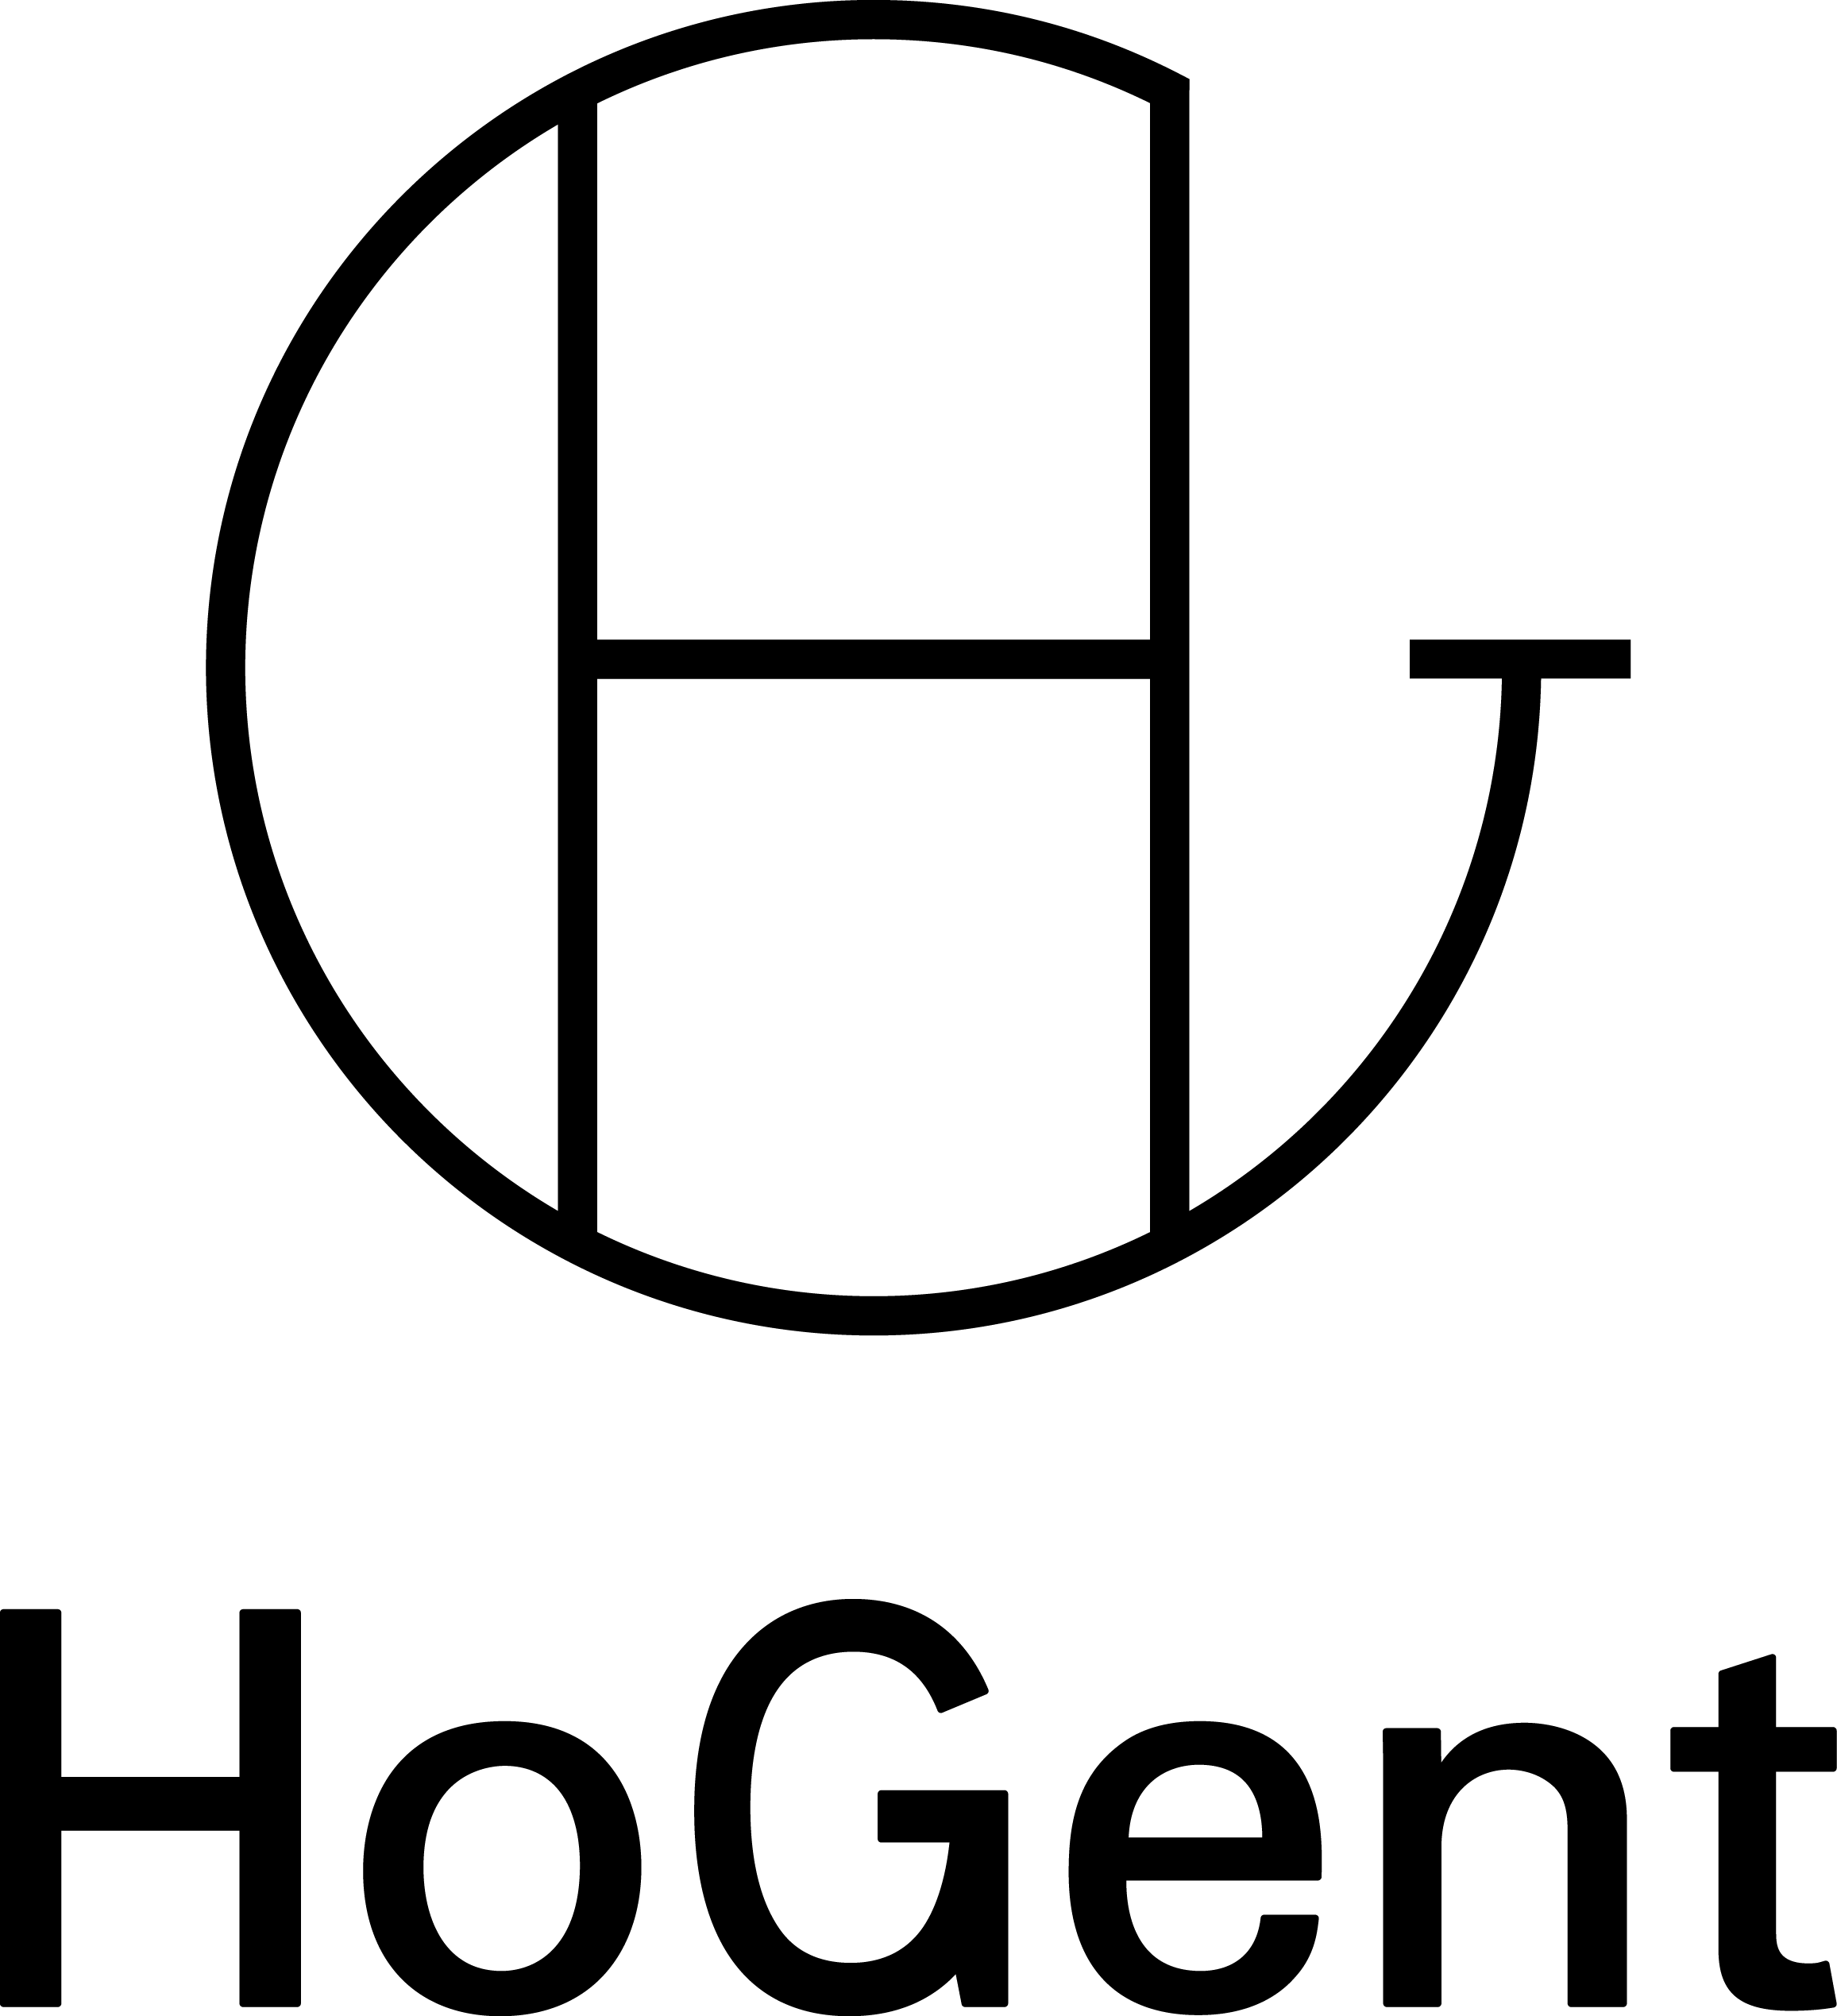
\includegraphics[width=2.5cm]{img/HG-beeldmerk-woordmerk}\\[.5cm]
    Faculteit Bedrijf en Organisatie\\[3cm]
    \titel
    \vfill
    \student\\[3.5cm]
    Scriptie voorgedragen tot het bekomen van de graad van\\professionele bachelor in de toegepaste informatica\\[2cm]
    Promotor:\\
    \promotor\\
    \ifdefempty{\copromotor}{\vspace{2.5cm}}{Co-promotor:\\\copromotor\\[2.5cm]}
    Instelling: \instelling\\[.5cm]
    Academiejaar: \academiejaar\\[.5cm]
    \ifcase \examenperiode \or Eerste \or Tweede \else Derde \fi examenperiode
    \endgroup

  \end{center}
  \restoregeometry
\end{titlepage}
  \emptypage
\begin{titlepage}
  \newgeometry{top=5.35cm,bottom=1.5cm,left=1.5cm,right=1.5cm}
  \begin{center}

    \begingroup
    \rmfamily
    \IfLanguageName{dutch}{Faculteit Bedrijf en Organisatie}{Faculty of Business and Information Management}\\[3cm]
    \titel
    \vfill
    \student\\[3.5cm]
    \IfLanguageName{dutch}{Scriptie voorgedragen tot het bekomen van de graad van\\professionele bachelor in de toegepaste informatica}{Thesis submitted in partial fulfilment of the requirements for the degree of\\professional bachelor of applied computer science}\\[2cm]
    Promotor:\\
    \promotor\\
    \ifdefempty{\copromotor}{\vspace{2.5cm}}{Co-promotor:\\\copromotor\\[2.5cm]}
    \IfLanguageName{dutch}{Instelling}{Institution}: \instelling\\[.5cm]
    \IfLanguageName{dutch}{Academiejaar}{Academic year}: \academiejaar\\[.5cm]
    \IfLanguageName{dutch}{%
    \ifcase \examenperiode \or Eerste \or Tweede \else Derde \fi examenperiode}{%
    \ifcase \examenperiode \or First \or Second \else Third \fi examination period}
    \endgroup

  \end{center}
  \restoregeometry
\end{titlepage}
}

%----------------------------------------------------------------------------------------
%	BIBLIOGRAPHY AND INDEX
%----------------------------------------------------------------------------------------

\usepackage[style=apa,backend=biber]{biblatex}
\usepackage{csquotes}
\DeclareLanguageMapping{dutch}{dutch-apa}
\addbibresource{bachproef-tin.bib} % BibTeX bibliography file
\addbibresource{../voorstel/biblio.bib}
\defbibheading{bibempty}{}

\usepackage{calc} % For simpler calculation - used for spacing the index letter headings correctly
\usepackage{makeidx} % Required to make an index
\makeindex % Tells LaTeX to create the files required for indexing

%----------------------------------------------------------------------------------------
%	MAIN TABLE OF CONTENTS
%----------------------------------------------------------------------------------------

\usepackage{titletoc} % Required for manipulating the table of contents

\contentsmargin{0cm} % Removes the default margin

% Part text styling
\titlecontents{part}[0cm]
{\addvspace{20pt}\centering\large\bfseries}
{}
{}
{}

% Chapter text styling
\titlecontents{chapter}[1.25cm] % Indentation
{\addvspace{12pt}\large\sffamily\bfseries} % Spacing and font options for chapters
{\color{maincolor!60}\contentslabel[\Large\thecontentslabel]{1.25cm}\color{maincolor}} % Chapter number
{\color{maincolor}}
{\color{maincolor!60}\normalsize\;\titlerule*[.5pc]{.}\;\thecontentspage} % Page number

% Section text styling
\titlecontents{section}[1.25cm] % Indentation
{\addvspace{3pt}\sffamily\bfseries} % Spacing and font options for sections
{\contentslabel[\thecontentslabel]{1.25cm}} % Section number
{}
{\hfill\color{black}\thecontentspage} % Page number
[]

% Subsection text styling
\titlecontents{subsection}[1.25cm] % Indentation
{\addvspace{1pt}\sffamily\small} % Spacing and font options for subsections
{\contentslabel[\thecontentslabel]{1.25cm}} % Subsection number
{}
{\ \titlerule*[.5pc]{.}\;\thecontentspage} % Page number
[]

% List of figures
\titlecontents{figure}[0em]
{\addvspace{-5pt}\sffamily}
{\thecontentslabel\hspace*{1em}}
{}
{\ \titlerule*[.5pc]{.}\;\thecontentspage}
[]

% List of tables
\titlecontents{table}[0em]
{\addvspace{-5pt}\sffamily}
{\thecontentslabel\hspace*{1em}}
{}
{\ \titlerule*[.5pc]{.}\;\thecontentspage}
[]

%----------------------------------------------------------------------------------------
%	MINI TABLE OF CONTENTS IN PART HEADS
%----------------------------------------------------------------------------------------

% Chapter text styling
\titlecontents{lchapter}[0em] % Indenting
{\addvspace{15pt}\large\sffamily\bfseries} % Spacing and font options for chapters
{\color{maincolor}\contentslabel[\Large\thecontentslabel]{1.25cm}\color{maincolor}} % Chapter number
{}
{\color{maincolor}\normalsize\sffamily\bfseries\;\titlerule*[.5pc]{.}\;\thecontentspage} % Page number

% Section text styling
\titlecontents{lsection}[0em] % Indenting
{\sffamily\small} % Spacing and font options for sections
{\contentslabel[\thecontentslabel]{1.25cm}} % Section number
{}
{}

% Subsection text styling
\titlecontents{lsubsection}[.5em] % Indentation
{\normalfont\footnotesize\sffamily} % Font settings
{}
{}
{}

%----------------------------------------------------------------------------------------
%	PAGE HEADERS
%----------------------------------------------------------------------------------------

\usepackage{fancyhdr} % Required for header and footer configuration

\pagestyle{fancy}
\renewcommand{\chaptermark}[1]{\markboth{\sffamily\normalsize\bfseries\chaptername\ \thechapter.\ #1}{}} % Chapter text font settings
\renewcommand{\sectionmark}[1]{\markright{\sffamily\normalsize\thesection\hspace{5pt}#1}{}} % Section text font settings
\fancyhf{} \fancyhead[LE,RO]{\sffamily\normalsize\thepage} % Font setting for the page number in the header
\fancyhead[LO]{\rightmark} % Print the nearest section name on the left side of odd pages
\fancyhead[RE]{\leftmark} % Print the current chapter name on the right side of even pages
\renewcommand{\headrulewidth}{0.5pt} % Width of the rule under the header
\addtolength{\headheight}{2.5pt} % Increase the spacing around the header slightly
\renewcommand{\footrulewidth}{0pt} % Removes the rule in the footer
\fancypagestyle{plain}{\fancyhead{}\renewcommand{\headrulewidth}{0pt}} % Style for when a plain pagestyle is specified

% Removes the header from odd empty pages at the end of chapters
\makeatletter
\renewcommand{\cleardoublepage}{
\clearpage\ifodd\c@page\else
\hbox{}
\vspace*{\fill}
\thispagestyle{empty}
\newpage
\fi}

%----------------------------------------------------------------------------------------
%	THEOREM STYLES
%----------------------------------------------------------------------------------------

\usepackage{amsmath,amsfonts,amssymb,amsthm} % For math equations, theorems, symbols, etc

\newcommand{\intoo}[2]{\mathopen{]}#1\,;#2\mathclose{[}}
\newcommand{\ud}{\mathop{\mathrm{{}d}}\mathopen{}}
\newcommand{\intff}[2]{\mathopen{[}#1\,;#2\mathclose{]}}
\newtheorem{notation}{Notation}[chapter]

% Boxed/framed environments
\newtheoremstyle{maincolornumbox}% % Theorem style name
{0pt}% Space above
{0pt}% Space below
{\normalfont}% % Body font
{}% Indent amount
{\small\bf\sffamily\color{maincolor}}% % Theorem head font
{\;}% Punctuation after theorem head
{0.25em}% Space after theorem head
{\small\sffamily\color{maincolor}\thmname{#1}\nobreakspace\thmnumber{\@ifnotempty{#1}{}\@upn{#2}}% Theorem text (e.g. Theorem 2.1)
\thmnote{\nobreakspace\the\thm@notefont\sffamily\bfseries\color{black}---\nobreakspace#3.}} % Optional theorem note
\renewcommand{\qedsymbol}{$\blacksquare$}% Optional qed square

\newtheoremstyle{blacknumex}% Theorem style name
{5pt}% Space above
{5pt}% Space below
{\normalfont}% Body font
{} % Indent amount
{\small\bf\sffamily}% Theorem head font
{\;}% Punctuation after theorem head
{0.25em}% Space after theorem head
{\small\sffamily{\tiny\ensuremath{\blacksquare}}\nobreakspace\thmname{#1}\nobreakspace\thmnumber{\@ifnotempty{#1}{}\@upn{#2}}% Theorem text (e.g. Theorem 2.1)
\thmnote{\nobreakspace\the\thm@notefont\sffamily\bfseries---\nobreakspace#3.}}% Optional theorem note

\newtheoremstyle{blacknumbox} % Theorem style name
{0pt}% Space above
{0pt}% Space below
{\normalfont}% Body font
{}% Indent amount
{\small\bf\sffamily}% Theorem head font
{\;}% Punctuation after theorem head
{0.25em}% Space after theorem head
{\small\sffamily\thmname{#1}\nobreakspace\thmnumber{\@ifnotempty{#1}{}\@upn{#2}}% Theorem text (e.g. Theorem 2.1)
\thmnote{\nobreakspace\the\thm@notefont\sffamily\bfseries---\nobreakspace#3.}}% Optional theorem note

% Non-boxed/non-framed environments
\newtheoremstyle{maincolornum}% % Theorem style name
{5pt}% Space above
{5pt}% Space below
{\normalfont}% % Body font
{}% Indent amount
{\small\bf\sffamily\color{maincolor}}% % Theorem head font
{\;}% Punctuation after theorem head
{0.25em}% Space after theorem head
{\small\sffamily\color{maincolor}\thmname{#1}\nobreakspace\thmnumber{\@ifnotempty{#1}{}\@upn{#2}}% Theorem text (e.g. Theorem 2.1)
\thmnote{\nobreakspace\the\thm@notefont\sffamily\bfseries\color{black}---\nobreakspace#3.}} % Optional theorem note
\renewcommand{\qedsymbol}{$\blacksquare$}% Optional qed square
\makeatother

% Defines the theorem text style for each type of theorem to one of the three styles above
\newcounter{dummy}
\numberwithin{dummy}{section}
\theoremstyle{maincolornumbox}
\newtheorem{theoremeT}[dummy]{Theorem}
\newtheorem{problem}{Problem}[chapter]
\newtheorem{exerciseT}{Exercise}[chapter]
\theoremstyle{blacknumex}
\newtheorem{exampleT}{Example}[chapter]
\theoremstyle{blacknumbox}
\newtheorem{vocabulary}{Vocabulary}[chapter]
\newtheorem{definitionT}{Definition}[section]
\newtheorem{corollaryT}[dummy]{Corollary}
\theoremstyle{maincolornum}
\newtheorem{proposition}[dummy]{Proposition}

%----------------------------------------------------------------------------------------
%	DEFINITION OF COLORED BOXES
%----------------------------------------------------------------------------------------

\RequirePackage[framemethod=default]{mdframed} % Required for creating the theorem, definition, exercise and corollary boxes

% Theorem box
\newmdenv[skipabove=7pt,
skipbelow=7pt,
backgroundcolor=black!5,
linecolor=maincolor,
innerleftmargin=5pt,
innerrightmargin=5pt,
innertopmargin=5pt,
leftmargin=0cm,
rightmargin=0cm,
innerbottommargin=5pt]{tBox}

% Exercise box
\newmdenv[skipabove=7pt,
skipbelow=7pt,
rightline=false,
leftline=true,
topline=false,
bottomline=false,
backgroundcolor=maincolor!10,
linecolor=maincolor,
innerleftmargin=5pt,
innerrightmargin=5pt,
innertopmargin=5pt,
innerbottommargin=5pt,
leftmargin=0cm,
rightmargin=0cm,
linewidth=4pt]{eBox}

% Definition box
\newmdenv[skipabove=7pt,
skipbelow=7pt,
rightline=false,
leftline=true,
topline=false,
bottomline=false,
linecolor=maincolor,
innerleftmargin=5pt,
innerrightmargin=5pt,
innertopmargin=0pt,
leftmargin=0cm,
rightmargin=0cm,
linewidth=4pt,
innerbottommargin=0pt]{dBox}

% Corollary box
\newmdenv[skipabove=7pt,
skipbelow=7pt,
rightline=false,
leftline=true,
topline=false,
bottomline=false,
linecolor=gray,
backgroundcolor=black!5,
innerleftmargin=5pt,
innerrightmargin=5pt,
innertopmargin=5pt,
leftmargin=0cm,
rightmargin=0cm,
linewidth=4pt,
innerbottommargin=5pt]{cBox}

% Creates an environment for each type of theorem and assigns it a theorem text style from the "Theorem Styles" section above and a colored box from above
\newenvironment{theorem}{\begin{tBox}\begin{theoremeT}}{\end{theoremeT}\end{tBox}}
\newenvironment{exercise}{\begin{eBox}\begin{exerciseT}}{\hfill{\color{maincolor}\tiny\ensuremath{\blacksquare}}\end{exerciseT}\end{eBox}}
\newenvironment{definition}{\begin{dBox}\begin{definitionT}}{\end{definitionT}\end{dBox}}
\newenvironment{example}{\begin{exampleT}}{\hfill{\tiny\ensuremath{\blacksquare}}\end{exampleT}}
\newenvironment{corollary}{\begin{cBox}\begin{corollaryT}}{\end{corollaryT}\end{cBox}}

%----------------------------------------------------------------------------------------
%	REMARK ENVIRONMENT
%----------------------------------------------------------------------------------------

\newenvironment{remark}{\par\vspace{10pt}\small % Vertical white space above the remark and smaller font size
\begin{list}{}{
\leftmargin=35pt % Indentation on the left
\rightmargin=25pt}\item\ignorespaces % Indentation on the right
\makebox[-2.5pt]{\begin{tikzpicture}[overlay]
\node[draw=maincolor!60,line width=1pt,circle,fill=maincolor!25,font=\sffamily\bfseries,inner sep=2pt,outer sep=0pt] at (-15pt,0pt){\textcolor{maincolor}{R}};\end{tikzpicture}} % Orange R in a circle
\advance\baselineskip -1pt}{\end{list}\vskip5pt} % Tighter line spacing and white space after remark

%----------------------------------------------------------------------------------------
%	SECTION NUMBERING IN THE MARGIN
%----------------------------------------------------------------------------------------

\makeatletter
\renewcommand{\@seccntformat}[1]{\llap{\textcolor{maincolor}{\csname the#1\endcsname}\hspace{1em}}}
\renewcommand{\section}{\@startsection{section}{1}{\z@}
{-4ex \@plus -1ex \@minus -.4ex}
{1ex \@plus.2ex }
{\normalfont\large\sffamily\bfseries}}
\renewcommand{\subsection}{\@startsection {subsection}{2}{\z@}
{-3ex \@plus -0.1ex \@minus -.4ex}
{0.5ex \@plus.2ex }
{\normalfont\sffamily\bfseries}}
\renewcommand{\subsubsection}{\@startsection {subsubsection}{3}{\z@}
{-2ex \@plus -0.1ex \@minus -.2ex}
{.2ex \@plus.2ex }
{\normalfont\small\sffamily\bfseries}}
\renewcommand\paragraph{\@startsection{paragraph}{4}{\z@}
{-2ex \@plus-.2ex \@minus .2ex}
{.1ex}
{\normalfont\small\sffamily\bfseries}}

%----------------------------------------------------------------------------------------
%	PART HEADINGS
%----------------------------------------------------------------------------------------

% numbered part in the table of contents
\newcommand{\@mypartnumtocformat}[2]{%
\setlength\fboxsep{0pt}%
\noindent\colorbox{maincolor!20}{\strut\parbox[c][.7cm]{\ecart}{\color{maincolor!70}\Large\sffamily\bfseries\centering#1}}\hskip\esp\colorbox{maincolor!40}{\strut\parbox[c][.7cm]{\linewidth-\ecart-\esp}{\Large\sffamily\centering#2}}}%
%%%%%%%%%%%%%%%%%%%%%%%%%%%%%%%%%%
% unnumbered part in the table of contents
\newcommand{\@myparttocformat}[1]{%
\setlength\fboxsep{0pt}%
\noindent\colorbox{maincolor!40}{\strut\parbox[c][.7cm]{\linewidth}{\Large\sffamily\centering#1}}}%
%%%%%%%%%%%%%%%%%%%%%%%%%%%%%%%%%%
\newlength\esp
\setlength\esp{4pt}
\newlength\ecart
\setlength\ecart{1.2cm-\esp}
\newcommand{\thepartimage}{}%
\newcommand{\partimage}[1]{\renewcommand{\thepartimage}{#1}}%
\def\@part[#1]#2{%
\ifnum \c@secnumdepth >-2\relax%
\refstepcounter{part}%
\addcontentsline{toc}{part}{\texorpdfstring{\protect\@mypartnumtocformat{\thepart}{#1}}{\partname~\thepart\ ---\ #1}}
\else%
\addcontentsline{toc}{part}{\texorpdfstring{\protect\@myparttocformat{#1}}{#1}}%
\fi%
\startcontents%
\markboth{}{}%
{\thispagestyle{empty}%
\begin{tikzpicture}[remember picture,overlay]%
\node at (current page.north west){\begin{tikzpicture}[remember picture,overlay]%
\fill[maincolor!20](0cm,0cm) rectangle (\paperwidth,-\paperheight);
\node[anchor=north] at (4cm,-3.25cm){\color{maincolor!40}\fontsize{220}{100}\sffamily\bfseries\@Roman\c@part};
\node[anchor=south east] at (\paperwidth-1cm,-\paperheight+1cm){\parbox[t][][t]{8.5cm}{
\printcontents{l}{0}{\setcounter{tocdepth}{1}}%
}};
\node[anchor=north east] at (\paperwidth-1.5cm,-3.25cm){\parbox[t][][t]{15cm}{\strut\raggedleft\color{white}\fontsize{30}{30}\sffamily\bfseries#2}};
\end{tikzpicture}};
\end{tikzpicture}}%
\@endpart}
\def\@spart#1{%
\startcontents%
\phantomsection
{\thispagestyle{empty}%
\begin{tikzpicture}[remember picture,overlay]%
\node at (current page.north west){\begin{tikzpicture}[remember picture,overlay]%
\fill[maincolor!20](0cm,0cm) rectangle (\paperwidth,-\paperheight);
\node[anchor=north east] at (\paperwidth-1.5cm,-3.25cm){\parbox[t][][t]{15cm}{\strut\raggedleft\color{white}\fontsize{30}{30}\sffamily\bfseries#1}};
\end{tikzpicture}};
\end{tikzpicture}}
\addcontentsline{toc}{part}{\texorpdfstring{%
\setlength\fboxsep{0pt}%
\noindent\protect\colorbox{maincolor!40}{\strut\protect\parbox[c][.7cm]{\linewidth}{\Large\sffamily\protect\centering #1\quad\mbox{}}}}{#1}}%
\@endpart}
\def\@endpart{\vfil\newpage
\if@twoside
\if@openright
\null
\thispagestyle{empty}%
\newpage
\fi
\fi
\if@tempswa
\twocolumn
\fi}

%----------------------------------------------------------------------------------------
%	CHAPTER HEADINGS
%----------------------------------------------------------------------------------------

% A switch to conditionally include a picture, implemented by  Christian Hupfer
\newif\ifusechapterimage
\usechapterimagetrue
\newcommand{\thechapterimage}{}%
\newcommand{\chapterimage}[1]{\ifusechapterimage\renewcommand{\thechapterimage}{#1}\fi}%
\def\@makechapterhead#1{%
{\parindent \z@ \raggedright \normalfont
\ifnum \c@secnumdepth >\m@ne
\if@mainmatter
\begin{tikzpicture}[remember picture,overlay]
\node at (current page.north west)
{\begin{tikzpicture}[remember picture,overlay]
\node[anchor=north west,inner sep=0pt] at (0,0) {\ifusechapterimage\includegraphics[width=\paperwidth]{\thechapterimage}\fi};
\draw[anchor=west] (\Gm@lmargin,-9cm) node [line width=2pt,rounded corners=15pt,draw=maincolor,fill=white,fill opacity=0.5,inner sep=15pt]{\strut\makebox[22cm]{}};
\draw[anchor=west] (\Gm@lmargin+.3cm,-9cm) node {\huge\sffamily\bfseries\color{black}\thechapter. #1\strut};
\end{tikzpicture}};
\end{tikzpicture}
\else
\begin{tikzpicture}[remember picture,overlay]
\node at (current page.north west)
{\begin{tikzpicture}[remember picture,overlay]
\node[anchor=north west,inner sep=0pt] at (0,0) {\ifusechapterimage\includegraphics[width=\paperwidth]{\thechapterimage}\fi};
\draw[anchor=west] (\Gm@lmargin,-9cm) node [line width=2pt,rounded corners=15pt,draw=maincolor,fill=white,fill opacity=0.5,inner sep=15pt]{\strut\makebox[22cm]{}};
\draw[anchor=west] (\Gm@lmargin+.3cm,-9cm) node {\huge\sffamily\bfseries\color{black}#1\strut};
\end{tikzpicture}};
\end{tikzpicture}
\fi\fi\par\vspace*{270\p@}}}

%-------------------------------------------

\def\@makeschapterhead#1{%
\begin{tikzpicture}[remember picture,overlay]
\node at (current page.north west)
{\begin{tikzpicture}[remember picture,overlay]
\node[anchor=north west,inner sep=0pt] at (0,0) {\ifusechapterimage\includegraphics[width=\paperwidth]{\thechapterimage}\fi};
\draw[anchor=west] (\Gm@lmargin,-9cm) node [line width=2pt,rounded corners=15pt,draw=maincolor,fill=white,fill opacity=0.5,inner sep=15pt]{\strut\makebox[22cm]{}};
\draw[anchor=west] (\Gm@lmargin+.3cm,-9cm) node {\huge\sffamily\bfseries\color{black}#1\strut};
\end{tikzpicture}};
\end{tikzpicture}
\par\vspace*{270\p@}}
\makeatother

%----------------------------------------------------------------------------------------
%	HYPERLINKS IN THE DOCUMENTS
%----------------------------------------------------------------------------------------

\usepackage{hyperref}
\hypersetup{hidelinks,backref=true,pagebackref=true,hyperindex=true,colorlinks=false,breaklinks=true,urlcolor= maincolor,bookmarks=true,bookmarksopen=false,pdftitle={Title},pdfauthor={Author}}
\usepackage{bookmark}
\bookmarksetup{
open,
numbered,
addtohook={%
\ifnum\bookmarkget{level}=0 % chapter
\bookmarksetup{bold}%
\fi
\ifnum\bookmarkget{level}=-1 % part
\bookmarksetup{color=maincolor,bold}%
\fi
}
}

%----------------------------------------------------------------------------------------
%	Java source code
%----------------------------------------------------------------------------------------

% Commando voor invoegen Java-broncodebestanden (dank aan Niels Corneille)
% Gebruik:
%   \codefragment{source/MijnKlasse.java}{Uitleg bij de code}
%
% Je kan dit aanpassen aan de taal die je zelf het meeste gebruikt in je
% bachelorproef.
\newcommand{\codefragment}[2]{ \lstset{%
  language=java,
  breaklines=true,
  float=th,
  caption={#2},
  basicstyle=\scriptsize,
  frame=single,
  extendedchars=\true
}
\lstinputlisting{#1}}

% Leeg blad
\newcommand{\emptypage}{%
\newpage
\thispagestyle{empty}
\mbox{}
\newpage
}


%%---------- Documenteigenschappen --------------------------------------------
%% TODO: Vul dit aan met je eigen info:

% Je eigen naam
\newcommand{\student}{Wouter Van Hecke}

% De naam van je promotor (lector van de opleiding)
\newcommand{\promotor}{Angeline Van Achter}

% De naam van je co-promotor. Als je promotor ook je opdrachtgever is en je
% dus ook inhoudelijk begeleidt (en enkel dan!), mag je dit leeg laten.
\newcommand{\copromotor}{Hadrien Van Durme}

% Indien je bachelorproef in opdracht van/in samenwerking met een bedrijf of
% externe organisatie geschreven is, geef je hier de naam. Zoniet laat je dit
% zoals het is.
\newcommand{\instelling}{Hogeschool Gent}

% De titel van het rapport/bachelorproef
\newcommand{\titel}{Hoe kan de blockchain technologie de problemen oplossen in verband met supply chain in de agricultuur?}

% Datum van indienen (gebruik telkens de deadline, ook al geef je eerder af)
\newcommand{\datum}{28 mei 2018}

% Academiejaar
\newcommand{\academiejaar}{2017-2018}

% Examenperiode
%  - 1e semester = 1e examenperiode => 1
%  - 2e semester = 2e examenperiode => 2
%  - tweede zit  = 3e examenperiode => 3
\newcommand{\examenperiode}{2}

%%=============================================================================
%% Inhoud document
%%=============================================================================

\begin{document}

%---------- Taalselectie ------------------------------------------------------
% Als je je bachelorproef in het Engels schrijft, haal dan onderstaande regel
% uit commentaar. Let op: de tekst op de voorkaft blijft in het Nederlands, en
% dat is ook de bedoeling!

%\selectlanguage{english}

%---------- Titelblad ---------------------------------------------------------
\inserttitlepage

%---------- Samenvatting, voorwoord -------------------------------------------
\usechapterimagefalse
%%=============================================================================
%% Voorwoord
%%=============================================================================

\chapter*{Woord vooraf}
\label{ch:voorwoord}

%% TODO:
%% Het voorwoord is het enige deel van de bachelorproef waar je vanuit je
%% eigen standpunt (``ik-vorm'') mag schrijven. Je kan hier bv. motiveren
%% waarom jij het onderwerp wil bespreken.
%% Vergeet ook niet te bedanken wie je geholpen/gesteund/... heeft
Dit is de bachelorproef met als onderwerp: 'Hoe kan de blockchain technologie de problemen oplossen in verband met supply chain in de agricultuur?'. Deze bachelorproef is geschreven in het kader van mijn laatste jaar Toegepaste informatica aan de Hoge School.\\*\\*Het voorbije jaar was ik al geïnteresseert in blockchain technologie, daarom zag ik deze bachelorproef ook als een perfecte kans om dieper in te gaan in bepaalde aspecten. Samen met mijn stage, dat ook over blockchain ging, heb ik al een redelijke basis dat mij verder kan helpen naar de toekomst.\\*\\*Graag zou ik volgende personen bedanken.\\*\\*
Ik zou graag als eerste mijn co-promotor, Hadrien Van Durme, bedanken voor het opvolgen en advies geven bij deze bachelorproef. Het is dankzij mijn co-promotor dat ik hyper ledger composer heb leren kennen en hier al een klein netwerk heb kunnen opstellen. Ook heeft hij mij geholpen deze bachelorproef zo correct mogelijk te houden.\\*\\*Tevens wil ik zeker ook mijn stage mentor Jens Mortier bedanken voor mij deze geweldige kans te geven om stage te lopen bij het bedrijf Trase en mij daardoor ook in de juiste richting te leiden.\\*\\*Ten slotte wil ik ook nog mijn promotor Angeline Van Achter bedanken als promotor en begeleider.

%%=============================================================================
%% Samenvatting
%%=============================================================================

% TODO: De "abstract" of samenvatting is een kernachtige (~ 1 blz. voor een
% thesis) synthese van het document.
%
% Deze aspecten moeten zeker aan bod komen:
% - Context: waarom is dit werk belangrijk?
% - Nood: waarom moest dit onderzocht worden?
% - Taak: wat heb je precies gedaan?
% - Object: wat staat in dit document geschreven?
% - Resultaat: wat was het resultaat?
% - Conclusie: wat is/zijn de belangrijkste conclusie(s)?
% - Perspectief: blijven er nog vragen open die in de toekomst nog kunnen
%    onderzocht worden? Wat is een mogelijk vervolg voor jouw onderzoek?
%
% LET OP! Een samenvatting is GEEN voorwoord!



%%---------- Nederlandse samenvatting -----------------------------------------
%
% TODO: Als je je bachelorproef in het Engels schrijft, moet je eerst een
% Nederlandse samenvatting invoegen. Haal daarvoor onderstaande code uit
% commentaar.
% Wie zijn bachelorproef in het Nederlands schrijft, kan dit negeren, de inhoud
% wordt niet in het document ingevoegd.

\IfLanguageName{english}{%
\selectlanguage{dutch}
\chapter*{Samenvatting}
\lipsum[1-4]
\selectlanguage{english}
}{}

%%---------- Samenvatting -----------------------------------------------------
% De samenvatting in de hoofdtaal van het document

\chapter*{\IfLanguageName{dutch}{Samenvatting}{Abstract}}

Technologie blijft maar evolueren. \\*\\*Bedrijven moeten mee met de tijd, anders worden ze achtergelaten en voorbij gestoken door andere bedrijven. Maar bedrijven hebben niet altijd de tijd / het vermogen om deze nieuwe technologieën te onderzoeken. Dit soort transformatie neemt veel tijd en geld in beslag. In de wereld van supply chain is dit niet anders, en met de opkomst van Blockchain zijn er heel veel mogelijkheden. Daarom is het belangrijk voor bedrijven dat gebruik van maken een supply chain, om deze mogelijkheden goed te onderzoeken om met een zo goed mogelijke uitkomst te komen. In deze bachelorproef is er gefocust op het bouwen van supply chain netwerk op een blockchain en hier bepaalde testen op uit te voeren.\\*\\* Natuurlijk is er eerst een literatuurstudie gedaan om kennis op te doen over aspecten zoals blockchain en supply chain. Alle stappen van literatuurstudie tot het bespreken van resultaten zijn te vinden in deze bachelorproef, zie het einde van de inleiding voor een duidelijke indeling hiervan. De conclusie van het onderzoek is dat het goed mogelijk is om blockchain technologie te combineren met supply chain, ookal is blockchain zelf nog in ontwikkeling en zal nog niet alles lukken. Deze technologie is nog lang niet perfect, dus het is belangrijk om hier aan te blijven werken en blijven onderzoeken. Een uitbreiding van het supply chain netwerk zou een goed begin zijn, het realiseren van een inlog systeem met het dynamisch aanmaken van producten bijvoorbeeld.

%---------- Inhoudstafel ------------------------------------------------------
\pagestyle{empty} % No headers
\tableofcontents % Print the table of contents itself
\cleardoublepage % Forces the first chapter to start on an odd page so it's on the right
\pagestyle{fancy} % Print headers again

%---------- Lijst figuren, afkortingen, ... -----------------------------------

% Indien gewenst kan je hier een lijst van figuren/tabellen opgeven. Geef in
% dat geval je figuren/tabellen altijd een korte beschrijving:
%
%  \caption[korte beschrijving]{uitgebreide beschrijving}

%\listoffigures
%\listoftables

% Als je een lijst van afkortingen of termen wil toevoegen, dan hoort die
% hier thuis. Gebruik bijvoorbeeld de ``glossaries'' package.
% https://www.sharelatex.com/learn/Glossaries

%%---------- Kern -------------------------------------------------------------

%%=============================================================================
%% Inleiding
%%=============================================================================

\chapter{Inleiding}
\label{ch:inleiding}

Technologie blijft evolueren, dit geldt voor alle sectoren. In deze bachelorproef wordt er dieper ingegaan in de sector van supply chain, meer specifiek voor de agricultuur. Deze technologie begint te verouderen, maar is zeer moeilijk om zomaar te gaan vervangen. De huidige supply chain management systemen zoals ERP en SAP brengen een paar problemen met zich mee, problemen waar een blockchain technologie wel hulp kan bieden. Deze problemen worden onderzocht en er wordt op een praktische manier naar een oplossing gezocht.
\\*\\*
Als praktische oplossing wordt een een fictief netwerk opgesteld dat een supply chain representeerd. Op dit netwerk zijn er bedrijven zoals winkels en fabrieken te vinden, net zoals de producten die ze kopen/verkopen. Natuurlijk kan dit netwerk zo uitgebreid mogelijk gemaakt worden, maar voor dit prototype hebben we het gehouden rond het proces van tomaten.
\\*\\*
Voor een bedrijf dat dit netwerk zou gebruiken, is de snelheid ervan ook een belangrijk onderdeel. Daarom worden er testen gehouden op de snelheid van het netwerk. Deze testen gaan van het aanmaken van producten tot het ophalen van 1 enkel product.

\section{Probleemstelling}
\label{sec:probleemstelling}

De bedoeling van deze bachelorproef is om bedrijven dat gebruik maken van supply chain, een prototype te tonen van hoe een supply chain eruit kan zien met een blockchain technologie. Dit kan gaan van bedrijven zoals Colruyt, waar het heel belangrijk is, ook naar de eindgebruiker toe, van waar het product precies komt, onder welke omstandigheden dat het getransporteert werd en natuurlijk hoe lang het product onderweg was met als laatste een van de belangrijkste vragen: Hoe lang blijven deze producten nog goed?

Aan de andere kant is deze bachelorproef ook handig voor IT-developers dat actief zijn in supply chain technologie. Dankzij dit prototype hebben ze een duidelijk beginpunt, het is dus bedoeling dat er verder kan gewerkt worden bovenop dit protoype.

\section{Onderzoeksvraag}
\label{sec:onderzoeksvraag}

'Hoe kan de blockchain technologie de problemen oplossen in verband met supply chain in de agricultuur?' Dit is de hoofdonderzoeksvraag. Er wordt gekeken naar de huidige problemen van een supply chain en hoe blockchain een rol kan spelen in het oplossen van deze problemen of hoe blockchain een meerwaarde kan zijn.

Deze hoofdonderzoeksvraag wordt nog eens onderverdeeld in drie kleinere deelvragen:

\begin{enumerate}
	\item \textbf{Hoe kan er met zekerheid gezegd worden dat de producten authentiek zijn?}\\*
	Bij deze vraag wordt er dieper op ingegeaan hoe men met zekerheid kan zeggen dat er niet gebeurt is met de producten dat niet mag en vooral aantonen van fabrieken deze producten deze producten komen. Wat tegenwoordig een heel belangrijk details is voor mensen.
	\item \textbf{Heeft het aantal gegevens op het netwerk een invloed op het ophalen en wegsturen van informatie?}\\*
	Zoals al eerder aangehaald werd, is het voor een bedrijf zeer belangrijk dat het netwerk optimaal is. Daarom is het handig als er enkele testen worden uitgevoerd op het netwerk.
	\item \textbf{Welke problemen kunnen niet opgelost worden met blockchain?}\\*
	Blockchain is op zich ook nog in ontwikkeling en zeker nog ver van perfectie. Daarom is het ook belangrijk om aan te halen welke aspecten niet / nog niet mogelijk zijn om met blockchain te realiseren.
\end{enumerate}

\section{Onderzoeksdoelstelling}
\label{sec:onderzoeksdoelstelling}

Er worden een paar zaken verwacht van de resultaten:

Voor de bevolking is het tegengaan van vervalsing en zekerheid hebben over hun producten topprioriteit. Dit gebeurt de dag van vandaag zeker niet altijd. Maar blockchain kan hier zeker een verandering in brengen. Omdat eens aangebrachte veranderingen voor altijd op de blockchain staat, kan dit door de eindpartij ook zelf bekeken worden of het inderdaad klopt wat er precies op het label staat.\\*\\*Er wordt verwacht van de resultaten van de testen dat deze snel zal zijn en dat er relatief gezien niet veel verschil zal zitten tussen testen met een groter aantal gegevens.\\*\\*Omdat blockchain zelf nog in zijn beginfase zit, zullen er waarschijnlijk ook wel aspecten zijn dat het nog niet kan oplossen. Supply chain zit ook heel complex in elkaar. Er zal naar de toekomst toe zeker nog heel veel werk in kruipen naar gelang implementatie toe.

\section{Opzet van deze bachelorproef}
\label{sec:opzet-bachelorproef}

De rest van deze bachelorproef is als volgt opgebouwd:

In Hoofdstuk~\ref{ch:stand-van-zaken} wordt een overzicht gegeven van de stand van zaken binnen het onderzoeksdomein, op basis van een literatuurstudie.

In Hoofdstuk~\ref{ch:methodologie} wordt de methodologie toegelicht en worden de gebruikte onderzoekstechnieken besproken om een antwoord te kunnen formuleren op de onderzoeksvragen.

In Hoofdstuk 4 wordt een introductie gegeven over Bitcoin, dit is een belangrijke basis om verder te gaan met blockchain.

In Hoofdstuk 5 wordt een introductie gegeven over blockchain, hier worden belangrijke concepten aangehaald wat belangrijk zal zijn voor bepaalde vragen.

In Hoofdstuk 6 wordt er gekeken naar wat een supply chain precies inhoud en wat de belangrijke aspecten hier in zijn.

In Hoofdstuk 7 worden de problemen van een supply chain onderzocht en gekeken hoe de blockchain op die vlakken kunnen helpen.

In Hoofdstuk 8 wordt uitleg gegeven over het gemaakte prototype met hyperledger composer. Hierin wordt er vertelt hoe het netwerk is opgemaakt met een demonstratie van de gemaakte mobile applicatie.

In Hoofdstuk 9 worden de testen besproken dat los gelaten worden op het netwerk met de uiteindelijke conclusie van de resultaten.

In Hoofdstuk 10 wordt besproken wat er verder onderzocht kan worden in de richting van supply chain gecombineerd met blockchain / welke andere testen er eventueel nog kunnen uitgevoerd worden.

In Hoofdstuk~\ref{ch:conclusie}, tenslotte, wordt de conclusie gegeven en een antwoord geformuleerd op de onderzoeksvragen. Daarbij wordt ook een aanzet gegeven voor toekomstig onderzoek binnen dit domein.


\chapter{Stand van zaken}
\label{ch:stand-van-zaken}

% Tip: Begin elk hoofdstuk met een paragraaf inleiding die beschrijft hoe
% dit hoofdstuk past binnen het geheel van de bachelorproef. Geef in het
% bijzonder aan wat de link is met het vorige en volgende hoofdstuk.

% Pas na deze inleidende paragraaf komt de eerste sectiehoofding.

\section{Blockchain + Supply chain}
In het eerste artikel ~\autocite{supchain1} wordt er informatie gegeven over wat de supply chain is en precies het doel is van supply chain management. Het geeft ook uitleg over wat de belemmeringen zijn van een supply chain en hoe de blockchain technologie in zijn tijd deze problemen kan helpen wegwerken. Een supply chain wordt omgeschreven als een sequentie van processen dat een product ondergaat. Een supply chain is alles behalve lineair, het is een netwerk van netwerken. De ene uitgang kan de ingang zijn van het volgende product. Maar het gaat niet alleen maar om de productstroom, ook over geldstroom, informatiestroom...\\*\\* Het belangrijkste van een supply chain is het beheren van de staat, dit kan gezien worden als de laatst geweten status van een proces of transactie. Deze dat wordt meestal ingegeven door meerdere bedrijven, zo kan het ontstaan het ene bedrijf informatie niet invult dat ergens anders wel ingevuld wordt. Zo onstaat er inconsistentie. Nog andere nadelen van de staat op dit moment is dat deze informatie niet real time zijn, er bestaat een vertraging tussen het uitwisselen van informatie tussen het digitale systeem en de fysieke supply chain. Deze informatie dat bijhouden wordt is heel bedrijfs centrisch gelegen. Er kan niet gekeken worden naar informatie buiten het eigen ERP systeem. Dit is namelijk het hoofdprobleem van ERP-systemen.\\*\\*Dit is alles behalve een netwerk van waarde, maar met de opkomst van de Blockchain technologie, samen met IoT en zelfs AI, kan dit allemaal veranderen in de toekomst. De huidige ERP systemen lijden aan een paar problemen dat kan worden opgelost met de blockchain technologie. Deze problemen zijn het manueel fouten maken bij het ingeven van gegevens en papierwerkfouten. De informatie ligt heel centrisch, maar het moet wel meerdere keren ingegeven worden door verschillende bedrijven. De aard van deze problemen ligt bij het feit dat bedrijven elkaar elkaar niet vertrouwen met hun informatie en daarom alles gecentreerd houden.\\*\\*Dankzij het opkomen van IoT, kan de informatie beheert en gecontroleerd worden in real time. Het automatiseren van processen kan vergemakkelijkt worden, terwijl dit wel voor meer transacties per seconden zorgt. De Blockchain technologie helpt daarnaast om één gedecentraliseerde database te verkrijgen, waar er transparantie ontstaat van de producten en processen. Dankzij de blockchain technologie kan er echt een netwerk van waarde worden opgesteld omdat de bedrijven elkaar niet hoeven te vertrouwen, het gedecentraliseerde netwerk zal het vertrouwen afdwingen.

\section{De agricultuur in China}
In het tweede artikel vertelt ~\textcite{agri1} over problemen in de agricultuur ter plaatse van China. Hij vertelt over de problemen van de boeren en de algemene problemen van de agricultuur. Het inkomen van de boeren is aan het zakken terwijl hun kosten alleen maar stijgen, terwijl de prijzen van het voedsel gedaald is en er minder vraag is van de middel klasse in China. De boeren hebben geen zekerheid tegen een grote ramp, zoals droogte en dat zo hun oogst niet zal slagen. Het land waarop ze werken is ook niet hun eigendom, ze huren dit van hun overheid. Hierdoor hebben ze weinig tot geen zeg over wat er moet gebeuren met het land in verband met verbeteringen. Ze hebben wel zelf de keuze wat ze planten, daar is er ook een moeilijkheid. Het is niet makkelijk om te voorspellen wat ze precies nodig hebben en hoeveel ze er van nodig hebben.\\*\\*Nu als het gaat over de gehele agricultuur in China, kan het volgende gezegd worden. Omdat de wegen en infrastructuur er zo slecht zijn, gebeurt het vaak dat de boer zijn producten niet op tijd bij de markten krijgt en ze daardoor rot aankomen. De kwaliteit van de producten zijn soms heel slecht of vervormd, door het gebruik van pesticiden en kunstmest. Vele landschappen zijn aan het uitdrogen of het landschap wordt onbruikbaar.

\section{Huidige problemen van een supply chain}
Het derde artikel ~\autocite{prob1} geeft een visie van welke huidige problemen er bestaan voor supply chain management. Maar eerst wordt er besproken wat een goede supply chain inhoud.\\*\\*Een supply chain moet de rauwe materialen kunnen bekijken, hierbij kan de supply chain manager het inplannen van nieuwe producten maken, effectieve inventaris opmaken om zoveel mogelijk kosten te verminderen en zich kunnen aanpassen aan de vraag van de consument. Alle informatie moet makkelijk verkrijgbaar zijn zodat er zich geen situaties voordoen als het moeten stopzetten van de productie. Een van de grootste problemen is dat de data real time moet zijn om een veel beter overzicht te krijgen van wat er allemaal gebeurt.\\*\\*Het eerste punt dat aangehaald wordt is de globalizering. Bedrijven verhuizen hun productiefabrieken meer naar het buitenland voor lagere kosten en minder belastingen, lagere transport kosten enzovoort. Maar dit brengt natuurlijk meer complexiteit binnen hun supply chain. De bedrijven moeten hun materialen meer organiseren en samen werken met andere bedrijven voor hun maken van producten, opslaan van het resultaat en het transport ervan.\\*\\*De markt is constant in beweging. Aankoop prijzen en verkoop prijzen veranderen constant, net zoals de vraag en het aanbod van de producten. De producten hebben een kortere levenscyclus, dit forceert de bedrijven om hun supply chain aan te passen. Het is moeilijk om te voorspellen hoeveel producten er precies moeten worden gemaakt, dat geldt dus ook voor hoeveel materiaal er moet worden aangekocht.\\*\\*Het laatste punt dat aangehaald wordt is de kwaliteit van de producten. Door de druk van sociale media moet er veel meer gekeken worden op consistente kwaliteit van de producten. Dit geldt voor het maken van het eindproduct, maar dit is ook belangrijk bij het aankopen van de rauwe materialen. De bedrijven moeten letten dat hun product tijdens de verwerking kwaliteitsvolle processen ondergaat, bv. tijdens het inpakken ervan, tijdens transportatie, zeker tijdens het kweken van eten zoals tomaten of granen.\\*\\*Tijdens deze processen moet er ook stevig wat papierwerk worden bijhouden. Dit is op zich al een heel makkelijk punt om fouten te maken. Een fout in het ingeven van gegevens kan al grote gevolgen hebben in het proces van het product. Er wordt ook rekening gehouden met documenten zoals vergunningen, licenties, certificaten.


%%Dit hoofdstuk bevat je literatuurstudie. De inhoud gaat verder op de inleiding, maar zal het onderwerp van de bachelorproef *diepgaand* uitspitten. De bedoeling is dat de lezer na lezing van dit hoofdstuk helemaal op de hoogte is van de huidige stand van zaken (state-of-the-art) in het onderzoeksdomein. Iemand die niet vertrouwd is met het onderwerp, weet er nu voldoende om de rest van het verhaal te kunnen volgen, zonder dat die er nog andere informatie moet over opzoeken \autocite{Pollefliet2011}.

%%Je verwijst bij elke bewering die je doet, vakterm die je introduceert, enz. naar je bronnen. In \LaTeX{} kan dat met het commando \texttt{$\backslash${textcite\{\}}} of \texttt{$\backslash${autocite\{\}}}. Als argument van het commando geef je de ``sleutel'' van een ``record'' in een bibliografische databank in het Bib\TeX{}-formaat (een tekstbestand). Als je expliciet naar de auteur verwijst in de zin, gebruik je \texttt{$\backslash${}textcite\{\}}.
%%Soms wil je de auteur niet expliciet vernoemen, dan gebruik je \texttt{$\backslash${}autocite\{\}}. In de volgende paragraaf een voorbeeld van elk.

%%\textcite{Knuth1998} schreef een van de standaardwerken over sorteer- en zoekalgoritmen. Experten zijn het erover eens dat cloud computing een interessante opportuniteit vormen, zowel voor gebruikers als voor dienstverleners op vlak van informatietechnologie~\autocite{Creeger2009}.

%%=============================================================================
%% Methodologie
%%=============================================================================

\chapter{Methodologie}
\label{ch:methodologie}

%% TODO: Hoe ben je te werk gegaan? Verdeel je onderzoek in grote fasen, en
%% licht in elke fase toe welke stappen je gevolgd hebt. Verantwoord waarom je
%% op deze manier te werk gegaan bent. Je moet kunnen aantonen dat je de best
%% mogelijke manier toegepast hebt om een antwoord te vinden op de
%% onderzoeksvraag.
\section{Literatuurstudie}
Voor deze bachelorproef is er een basis nodig aan kennis van bepaalde termen, waar onder blockchain en supply chain. Om verder te gaan met het onderzoek moesten deze termen eerst onderzocht worden aan de hand van een literatuurstudie. Bitcoin was de eerste term dat onderzocht werd, omdat het daar eigenlijk allemaal begonnen in. Bij het onderzoeken van blockchain hoort dus ook wat onderzoek naar het ontstaan van Bitcoin. Hierbij werden verschillende artikels bekeken om kennis te vergaren over Bitcoin. Vervolgens was blockchain aan de beurt, om hier informatie over te verkrijgen was onder andere het boek Blockchain Basics benut. In dit boek stonden er aspecten wat de term blockchain precies inhoud en wat het wil bereiken. Ook was er informatie te vinden hoe het op een abstract level inhoudelijk in elkaar zit, wat een goed zicht gaf om te begrijpen wat blockchain precies is en hoe het best gebruikt kan worden.\\*\\*
Daarna was het de beurt aan supply chain. Hierbij werd er in het begin onderzocht wat supply chain en supply chain management precies inhouden. Dan kwamen de problemen van een supply chain. Omdat blockchain al onderzocht was, kon er op het einde van de literatuurstudie al geantwoord worden op de vraag wat welke problemen een blockchain (nog) niet kan oplossen.

\section{Prototype}
Als tweede deel werd een prototype gemaakt van een supply chain op een blockchain. Hiervoor waren er 2 opties: Ethereum en Hyperledger composer. Met Ethereum zou er een smart contract gemaakt worden om zo het netwerk te simuleren. Maar Hyperledger composer is specifiek bedoeld om netwerken op te bouwen. Daarom lag de keuze al snel bij Hyperledger composer. Als eerste werd er een netwerk bedacht dat bestaat uit bedrijven en producten. Omdat de focus hier gelegd werd bij agricultuur, zullen de producten gesimuleerd worden als tomaten. Er werden verschillende soorten bedrijven gekozen dat elk met hun eigen producten werkten, bijvoorbeeld lasagna of spaghetti saus, dat dus ook gemaakt wordt van tomaten. Om deze gegevens op het netwerk te zetten, moet er wel eerst een netwerk zijn. Dit netwerk opstellen was ook helemaal nieuw, dus moest er onderzocht worden hoe dit precies in elkaar zat. In de loop van dit prototype werd er een Hyperledger composer netwerk opgesteld dat het netwerk simuleerde, een NodeJS applicatie dat de informatie regelde van het netwerk en een mobiele applicatie dat met dit netwerk kon communiceren. Hoe dit netwerk met de applicaties werden opgesteld, komt verder aan bod in Hoofdstuk 8.

\section{Testen}
Ten slotte, werden er enkele testen geschreven dat werken uitgevoerd op het netwerk. De snelheid van een netwerk is heel belangrijk voor een bedrijf dat dit netwerk gebruikt. Omdat deze testen lijken op de NodeJS applicatie, zijn er stukken code uit de applicatie gehaald en hergebruikt. Deze testen kunnen dus ook gezien worden als NodeJS scripts. Omdat het prototype gemaakt was in een virtuele machine, had het netwerk ook zo zijn limitaties. Daarom konden sommige testen spijtig genoeg niet uitgevoerd worden omdat ze te lang duurde en het netwerk dit niet aankon. Hierbij horen de testen van het verwijderen van veel gegevens. Alle (andere) testen werd uitgevoerd met een verschillend aantal gegevens, met de bedoeling om te kijken of het aantal gegevens dat zich op het netwerk bevond, een groot verschil uitmaakte voor de snelheid van de transacties. Hieronden bevinden zich alle testen dat zijn uitgevoerd:\\*
\begin{enumerate}
	\item Creatie van informatie
	\item Verwijderen van informatie
	\item Ophalen van alle producten / bedrijven
	\item Opzoeken van één bepaalde ID
\end{enumerate}



% Voeg hier je eigen hoofdstukken toe die de ``corpus'' van je bachelorproef
% vormen. De structuur en titels hangen af van je eigen onderzoek. Je kan bv.
% elke fase in je onderzoek in een apart hoofdstuk bespreken.

%\input{...}
%\input{...}
%...
\chapter{Bitcoin}
Voordat we beginnen met de hoofdzaken, is het belangrijk dat we eerst de terminologie rond blockchain goed snappen. Vandaar deze intro over Bitcoin en blockchain.

%%De oorsprong van Bitcoin
\section{De historiek van Bitcoin}
Het onstaan van Bitcoin gaat helemaal terug tot in 2008, toen een mysterieuze persoon genaamd Satoshi Nakamoto een paper ~\autocite{bit1} uitbracht onder de titel: "Bitcoin, a peer to peer electronic cash system".Wie deze persoon precies is, is tot op deze dag nog altijd niet gekend. Satoshi Nakamoto is in 2011 van het internet verdwenen.\\*\\*In het jaar 2009 werd voor het eerst het gedecentraliseerde Bitcoin system publiek gemaakt. Dit hield in dat mensen bitcoins konden minen - een wiskundig proces waarbij nieuwe bitcoins worden gecreeërd - als ook transacties versturen en verifiëren op de Bitcoin blockchain. Meer over blockchain in het volgende hoofdstuk.\\*\\* In het jaar 2010 kreeg een bitcoin voor de eerste keer een waarde, er werden maar liefst 10 000 bitcoins ingewisseld voor 2 pizza's. Op het moment van het schrijven van deze bachelorproef, zou dat een waarde hebben van 60 miljoen euro. Dit lijkt nu een belachelijk groot bedrag, maar dit moment was ook heel memorabel in de geschiedenis van bitcoin. Het was de allereerste keer dat er een echt product werd gekocht en dus dat bitcoin voor de eerste keer als een echt betaalmiddel gebruikt werkt. \\*\\*Er werd meer en meer interesse getoond in deze gedecentraliseerde technologie, er kwamen nieuwe projecten boven water met het doel om de Bitcoin blockchain te verbeteren. Deze projecten hebben ook hun eigen coin of token, een paar bekende voorbeelden zijn: de Ethereum blockchain met hun coin genaamd Ether, de Ripple blockchain met hun coin genaamd XRP. Er zijn in totaal meer dan 1000 van deze coins, meestal worden ze onder een overkoepelende term gezet, namelijk altcoins.\\*\\*Een blockchain draait vooral rond het decentraliseren van centrale systemen en het oplossen van het vertrouwensprobleem tussen verschillende partijen. Op dit punt in tijd stond de beveiliging nog niet helemaal op peil en bestaan er nog altijd kwetsbaarheden in het netwerk. Omdat bitcoin op dat moment redelijk nieuw was en een digitale waarde voorstelde, was dit ook een doelwit voor hackers. In het jaar 2014 gaat de bekende site Mt. Gox offline nadat ze gehacked waren en er maar liefst 850,000 bitcoins gestolen werden, wat nu een waarde zou hebben van maar liefst 5.1 miljard euro.\\*\\*Maar zelfs dat hield Bitcoin niet tegen, over de jaren heeft het als maar meer en meer aandacht gekregen en is de waarde blijven stijgen. In het jaar 2016 kwam er een nieuw concept genaamd ICO's of wel "Initial coin offering", ook vergelijkbaar met crowdfuncing of "IPO". Start up bedrijven konden op deze manier hun initieel bedrag verkrijgen en de mensen die hun geld gaven coins in de plaats geven. Die coins hebben op zich ook een waarde dat kan zakken of stijgen.\\*\\*Tot op de dag van vandaag is bitcoin blijven stijgen in waarde tot op een hoogtepunt van 18 000 euro.
~\autocite{hist1}

%%Voor- en nadelen van bitcoin
\section{Voor- en nadelen van bitcoin}
Sommige aspecten van Bitcoin kunnen zowel als positief als negatief aanzien worden. voorbeelden hiervan zijn: transactiesnelheid, privacy, controle...
\\*\\*
\textbf{Voordelen}\\*\\*
Omdat er geen centrale autoriteit is op een blockchain ben je onafhankelijk van banken of de overheid. Bitcoin is een globale munt waar je dus overal met kan betalen.\\*Het verwerkingsproces van het verzenden op de Bitcoin blockchain is in vergelijking met het huidige banken systeem veel sneller. Als je een transactie wil uitvoeren bij een bank, kan dit gemakkelijk 3 dagen duren. Bij Bitcoin zal dit ongeveer gebeuren in 1 uur. Er zijn al projecten zoals Ripple of NEO waar de transactieduur verminderd werd tot een paar seconden/minuten.\\*Omdat je altijd in het bezit bent van je eigen coins, heb je zelf de complete controle, indien je de coins veilig houdt in een wallet. Niemand kan aan deze coins behalve de persoon die in het bezit is van de privé sleutel. Meer informatie over wallets in het volgende hoofdstuk.\\*Als er transacties gebeuren op een blockchain weet niemand wie je bent, wat ze wel kunnen zien is bijvoorbeeld van welk adres de bitcoins komen en naar welk ander adres ze verstuurd wordt. Er werd dus een pseudo-anonimiteit op de blockchain ontwikkeld waar niemand uw identiteit precies kent.
\\*\\*\textbf{Nadelen}\\*\\*
Aan bijna elk voordeel zit er ook een nadeel.\\*Omdat er altijd maar meer en meer mensen het Bitcoin netwerk toetreden, wordt het alsmaar duurder en langer voor een transactie uit te voeren, meer uitleg over blockchain transacties in het hoofdstuk van Blockchain.\\*Omdats sommige blockchains volledig anoniem zijn, is het veel makkelijker om deze coins te gebruiken voor het aankopen van drugs en wapens op de zwarte markt, omdat je veel moeilijker op te sporen bent.\\* Er is geen centraal controlepunt door een overheid bijvoorbeeld, maar dat wil niet zeggen dat ze zich er niet met bemoeien. In vele landen wordt er al gesproken over het invoeren van belastingen op de winst dat je krijgt als je belegd in coins. Ze zullen dit ook proberen reguleren, wat dus eigenlijk het overgestelde is van wat een blockchain wil zijn.\\*Volledige controle over je eigen geld is natuurlijk heel goed, maar wat gebeurt er als er iets fout gaat? Je staat er helemaal alleen voor want er is niemand waar je naar toe kunt voor hulp. Je moet dus altijd heel voorzichtig zijn met wat je doet met je geld.  
~\autocite{voor1}

\section{Wallets}
Als je in het bezit wil zijn van je eigen coins, zal je deze moeten opslaan in je eigen wallet. Er zijn er paar verschillende wallets zoals een "cold storage wallet", een 'paper wallet' of een "web wallet". Bij het aanmaken van een nieuwe wallet krijg je 3 belangrijke gegevens: een adres, een publieke sleutel en een private sleutel. Met je private sleutel krijg je toegang tot je geld terwijl je publieke sleutel openlijk bekend staat op de blockchain. Meer informatie over beide sleutels in de blockchain hoofdstuk.\\* Elke wallet heeft zijn eigen adres, dat gebruikt wordt en geld naar overzetten. Stel dat persoon A 5 bitcoins naar persoon B wil sturen, dan zal persoon A dit naar het adres van persoon B sturen.\\*\\*Er bestaan een paar verschillende wallets die hier kort besproken zullen worden:\\*\\*
\textbf{Online web wallet}\\*\\*
Een voorbeeld van een 'web wallet' is MetaMask. Dit is een wallet dat je kan openen in een webbrowser.
\\*\\*\textbf{Software wallet}\\*\\*
Een software wallet is een wallet dat je zal draaien op je eigen computer en zo je coins kan beheren. Een voorbeeld van een software wallet is Exodus.
\\*\\*\textbf{Hardware wallet}\\*\\*
Een hardware wallet kan je vergelijken met een usb stick, speciaal geprogrammeerd als wallet. Het voordeel van een hardware wallet is dat je private sleutel nooit het apparaat verlaat en dus ook niet met het internet verbonden is tot zo lang dat je er niet zelf met connecteert. Een hardware wallet is de aangeraden optie voor mensen dat al een groter bedrag hebben.
\\*\\*\textbf{Paper wallet}\\*\\*
Met een 'paper wallet' zal je de publieke en private sleutel afdrukken om een papier en zo bijhouden. Dit stukje papier is dan de enige toegang dat je hebt tot je geld.
~\autocite{wallet1}
\section{Anoniemiteit}
Op een blockchain blijft een persoon normaal pseudo-anoniem tot dat deze persoon onderheven wordt aan het proces van "Know your customer". Er zijn wel blockchains waar een persoon helemaal anoniem kan zijn, bv op de blockchain van Monero. Op sommige exchange site of uitwisselingsite moeten mensen hun gegevens invullen voordat ze cryptocurrency kunnen kopen. Dit is een website waar je verschillende coins kan kopen en verkopen. Maar voordat je dat kan doen, moet je eerst geregistreerd staan op hun database. De coins die op de exchange staan, heb je dus zelf niet in eigen bezit, maar ze zijn wel in het bezit van de exchange, omdat deze exchange in het bezit is van de privé sleutel van de persoon in kwestie.

%%De derde partij
\section{De derde partij}
Een van de zaken dat een blockchain kan doen is de man in het midden wegwerken. Het grootste voorbeeld is nu een bank. De mogelijk om geld snel en goedkoop naar iemand te versturen zonder dat je moet rekenen op een bank is gigantisch. Omdat een blockchain een peer to peer systeem is, bestaat er een connectie van persoon A naar persoon B zodat er geen tussen persoon nodig is.

\chapter{De blockchain technologie}
~\autocite{blockchain1}

\section{Wat is blockchain?}
\textbf{Verschil gecentraliseerd / gedecentraliseerd netwerk}\\*\\*
Bij het maken van een software systeem, kom je voor de keuze te staan over de architectuur van het netwerk, dit kan zowel centraal als decentraal. Deze twee zijn de belangrijkste architecturen. Bij een centraal netwerk zal er altijd een centraal component aanwezig zijn waar al het verkeer naartoe lijdt. Dit maakt het ook een makkelijk doelwit voor hackers. Als het lukt om het centrale punt neer te halen, ligt heel het netwerk plat. In vergelijking met een gedecentraliseerd netwerk waar er geen centreel punt is, het netwerk blijft runnen ookal wordt er 1 component (of node) uit het systeem wordt gehaald. In een gedecentraliseerd systeem is elke node indirect met elkaar verbonden, dat wil niet zeggen dat elke node met elk andere node verbonden zal zijn, maar via via er wel een connectie met heeft.\\* \\*

Dit zijn de voordelen van een blockchain:\\*\\*
Het grootste voordeel van een blockchain is het oplossen van het vertrouwensprobleem. Partijen vertrouwen elkaar meestal niet, er komt nog een derde partij tussen dat de twee andere partijen wel vertrouwen dat alles vertrouwbaar verloopt. Deze derde partij vraag hier ook geld voor. Een blockchain zorgt ervoor dat deze derde partij niet meer nodig is door de manier hoe een blockchain systeem wordt opgesteld.\\*
In vergelijking met een centraal systeem, waar de kracht meestal uit een (super) computer wordt gehaald, wordt de kracht in een gedecentraliseerd systeem gehaald uit de combinatie van alle nodes in het netwerk. Hierdoor is de rekenkracht meestal veel groter.\\*\\*Alhoewel de initiële kost voor het opzetten van de gedecentraliseerd systeem hoger ligt dan bij een gecentraliseerd systeem, op langer termijn zal je nog altijd veel kosten bespraren omdat het veel duurder is om een (super / centrale) computer te beheren en onderhouden. Het is ook veel makkelijker om in een gedecentraliseerd systeem een computer te vervangen.\\*\\*Als er in een gedecentraliseerd netwerk één van de computers crasht, heeft dit weinig gevolgen op het volledige netwerk.\\*\\*Door het toevoegen van meer computers in het netwerk, verhoog je de rekenkracht van het hele netwerk. Daarom is er een natuurlijk vermogen om het netwerk uit te breiden. Hierdoor zijn er wel meer ingangen tot inbraak in het netwerk.\\*\\*

Natuurlijk heeft een gedecentraliseerd systeem ook zijn nadelen:\\*\\*In een gedecentraliseerd netwerk is er geen coördinatie door een centraal punt, daarom moet er rekenkracht opzij gehouden worden zodat elke node dit zelf kan doen. Niet zomaar elke node is goed genoeg voor het netwerk, zo moet een node voldoen aan een minium specificatie om zich te kunnen voorstellen als een node van het netwerk.\\*\\*Coördinatie vereist communicatie, dit moeten de nodes ook zelf doen.\\*\\*Een geschreven software voor op een gedecentraliseerd systeem moet nog een paar extra taken vervullen. Namelijk de nadelen dat hierboven beschreven staan. Hierdoor worden de programma's veel complexer omdat natuurlijk alle nodes over een en dezelfde informatie moet beschikken.\\*\\*In een publieke blockchain kan iedereen toetreden, hierdoor is er niet geweten of elke node te betrouwen in. Deze onbetrouwbare node zouden verkregen informatie kunnen vervalsen en terug doorsturen. Hierdoor zal er dus een stevige beveiliging aanwezig moeten zijn in het programma. In vergelijking met een private blockchain waar de node moet toegelaten worden door fundament dat de private blockchain heeft opgericht.

\textbf{Integriteit, een heel belangrijk aspect van een blockchain}\\*\\*
Integriteit. Voor een blockchain staat integriteit op nummer 1. Een blockchain kan aanzien worden als een instrument voor het bekomen en onderhouden van de integriteit van een decentraliseerd systeem. Maar wat bedoeld men nu precies?\\*Het is een heel belangrijk niet-functioneel aspect van een software programma, de gebruikte data moet correct en volledig zijn, het programma moet op een correcte manier werken / niet vast lopen en de gegevens mogen altijd maar toegankelijk zijn voor de mensen dat daadwerkelijk toegang hebben. Als deze waarden geschonden worden, kan dit grote gevolgen hebben voor de gebruikers. Een voorbeeld is bij het vast lopen van een excel bestand terwijl er niet opgeslagen werd. De programmeurs doen er alles aan om dit zoveel mogelijk te verkomen en moest het wel gebeuren, ten minste de data veilig te stellen. Zodra er data wordt weggeschreven naar ee blockchain, staat dit er voor altijd op. Stel dat er een programma wordt opgezet en hier zitten fouten in. Dan staat dit ook fout op de blockchain en kan dit niet meer angepast worden.\\*\\*
\textbf{Hoe ziet een blockchain er nu eigenlijk uit?}\\*\\*
Je kan een blockchain letterlijk zien als een ketting van blokken. In elke blok zitten de gegevens van alle transacties die in het verleden tot op het heden al gebeurd zijn. Deze gegevens zijn niet te vervalsen dankzij het gebruik van hash-functies, meer daarover in één van de volgende hoofdstukken. Elke node in het netwerk probeert de eerste te zijn dat een nieuwe block kan maken, vanaf er iemand een blok gemaakt, moeten al de andere nodes stoppen met hun blok en de gemaakte blok verifiëren op correctheid. Als deze blok inderdaad correct is, nemen ze deze op in hun geschiedenis en proberen ze terug de volgende block te creëren of met andere woorden "minen".

\textbf{Terminologie van een blockchain?}\\*\\*
Een blockchain kan gezien worden als een data structuur. Het is een manier van data te organiseren. De data wordt opgeslaan in een blok en elke blok wordt met elkaar geconnecteerd. De ordering waarin dit gebeurt is van groot belang. Stel dat er bitcoin uitgewisseld worden over 4 adressen, dan wil je de juiste volgorde weten van welk adres het kwam en naar waar het gaat, en zeer belangrijk, wie dus de eigenaar is.\\*Een blockchain kan ook gezien worden als een algoritme, het gaat hem hier dan over de sequentie van instructies dat er op het netwerk gebeurt in verband met creëren van een blok, verifiëren van een blok, de juiste historiek kiezen...\\*De blockchain technologie wordt anderzijds ook aanzien als een soort van overkoepelende mantel van verschillende zaken, zoals de combinatie van de data structuur, het algoritme, maar zowel van cryptografie dat instaat voor eigendom op de blockchain en de beveiliging voor op het gedecentraliseerde netwerk.

\section{Eigendom / Identicatie / Authenticatie / Authorisatie}
Een kernbegrip van een blockchain gaat over de eigendom. Weten wie de eigenaar is en van wat de persoon de eigenaar is. Maar hoe wordt er nu bepaald wie een eigenaar is. Stel dat deze informatie zich bevindt op één plaats, dan hebt je één punt dat je moet vertrouwen. Dit doet een blockchain anders. Op een blockchain wordt deze informatie op meerdere plaatsen opgeslaan en wordt er dus gekeken naar de wet van meederheid. Stel dat er acht van de tien nodes zeggen dat transactie A correct is en de andere twee nodes zeggen dat transactie A niet correct is, dan is er meer kans de transactie A inderdaad klopt. Dit concept is te vergelijken met een rechtbank, waar er meerdere mensen een beslissing moeten maken in plaats van één.
\\*\\*\textbf{Het kunnen bewijzen van de eigendom}\\*\\*
Het bewijzen van activieten van een persoon gebeurt via een signature. Elke persoon heeft een privé sleutel en een publieke sleutel. Als deze persoon een bericht of transactie encrypteert met zijn privé sleuten, is dit bericht alleen maar decrypteerbaar met de publieke sleutel van die persoon. Zo weet men met zekerheid dat de persoon in kwestie daadwerkelijk het bericht heeft gestuurd. Hierover meer bij het gedeelte van cryptografie.
\\*\\*\textbf{Identicatie / Authenticatie / Authorisatie}\\*\\*
Identificatie betekent het beweren van wie je bent. Bijvoorbeeld zeggen dat Jan noemt. Hier komt er nog niets te pas van hoe je dit gaat bewijzen.
\\*Authenticatie betekent het bewijzen van wie je bent. Bijvoorbeeld je rijbewijs voorleggen.
\\*Authorisatie betekent het toegang krijgen tot iets waar je voor moest bewijzen dat je daadwerkelijk toegang had. Bijvoorbeeld een persoon dat 18+ moet zijn om te mogen rijden. Dit kunnen we ook reflecteren naar de blockchain technologie. Op een blockchain is iedereen uniek, ze worden gescheiden van elkaar, niet door een naam, maar wel door een privé sleutel. Meer over private sleutels later. Het authenticatie gedeelte op de blockchain wordt afgehandeld met behulp van "two-way hashing". Dit is een combinatie van je privé sleutel, je publieke sleutel en hash-functies. Meer hierover in het deel over hashing.\\*\\*
Integriteit op een blockchain heeft dus onder andere te maken over echte uitspraken over eigendommen.
\section{'Double spend' probleem}
Een van de meest schendende voorbeelden van de integriteit is het 'Spending money twice' probleem.
\\*\\*\textbf{Wat is het probleem?}\\*\\*
De informatie over de eigendom staat op elke node in het netwerk opgeslaan. Als er één verandering gebeurt van deze informatie, moeten alle andere nodes dit ook weten. Maar dit neemt natuurlijk tijd in, dus zal de blockchain in een status komen waarvoor er nodes zijn die de nieuwe informatie al kennen wanneer dat nog niet zo is bij andere nodes. Dit zou gemanipuleerd kunnen worden door de eigenaar van bijvoorbeeld een auto. Stel nu dat de eigenaar van een auto 'persoon A', zijn auto wil verkopen aan 'persoon B' en dus de eigendom doorgeven. Vanaf deze auto doorgegeven wordt en de nodes bezig zijn met het aanpassen van hun informatie, kan 'persoon A' naar een andere node gaan waar de informatie nog niet is toegekomen en daar de auto verkopen aan 'persoon C'. Dit is het probleem dat wordt gezien als het 'spending money twice' probleem.
\\*\\*\textbf{Hoe wordt dat probleem opgelost?}\\*\\*
Om dit probleem op te lossen wordt dus de technologie van de blockchain gebruikt. Dit zal duidelijker worden aan de hand van volgende deelhoofdstukken.
\section{Hashing}
Op een blockchain krijg je te maken met heel veel data, deze data moet je op een snelle en efficiënte manier uniek maken en kunnen vergelijken. Vandaar dat er hier hashing wordt toegepast. Hash functies zijn kleine programma's dat eender welke data als input krijgt en die data verandert in een combinatie van hexadecimale getallen.
\\*\\*\textbf{Aspecten van cryptografische hash functies}\\*\\*
Bij het gebruik van cryptografische hash functies, zijn de hash values altijd uniek. Identieke input zal altijd een identieke hash value geven.\\*De output is pseudorandom, dat betekent dat de output van een bijna identieke input, veel verschil kan hebben.\\*Een hashing functie is een 'one-way functie', dat betekent dat je bijna onmogelijk van de output terug naar de input kan gaan.\\*Er zijn miljoenen verschillende combinatie van hash values, dus de kans dat er twee keer dezelfde hash value wordt gevonden voor een identieke input is immens klein.
\\*\\*\textbf{Een voorbeeld van hashing}~\autocite{blockchain1}\\*\\*
\begin{center}
	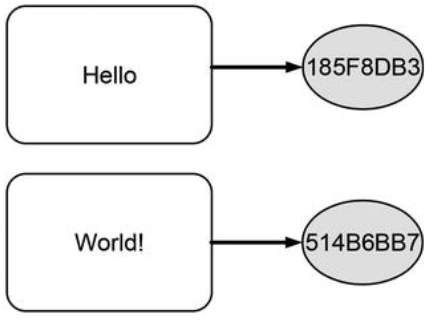
\includegraphics[width=10cm]{img/hashing}\\[1cm]
\end{center}
\textbf{Verschillende hash patronen}\\*\\*
Het eerste en simpelste voorbeeld is onafhankelijk hashen. In dit partoon wordt van elke data individueel de hash value berekend.\\*\\*In het volgende voorbeeld bespreken we het herhaald hashen. In dit partoon wordt de input eerst gehashed, en daarna wordt de hash value nog eens gehashed. Dit is mogelijk omdat een hash value ook een vorm van data is en daarom kan dienen als input.\\*\\*Het volgende partoon gaat over combinerend hashen. Stel dat we 2 inputs willen hashen met het combinerend hashing partoon, dan zal als eerste de input aan elkaar geplakt worden. Daarna wordt er één hash value gecreëerd van de gecombineerde input. Een nadeel aan dit patroon is dat de hash value van de individuele inputs niet gekent is.\\*\\*Het sequentieel hashing patroon, Dit is een combinatie van de het herhaalde hashing patroon en het combinerende hashing patroon.De eerste input zal gehashed worden. Deze hash value zal gecombineerd worden met de volgende input, wat op zijn beurt weer een nieuwe hash value geeft. Zo zal dit proces blijven door gaan tot dit compleet is.\\*\\*Als laatste patroon bespreken we het hiërarchische hashing patroon ofwel een Merkle Tree genoemd dat te zien is in de onderstaande foto ~\autocite{blockchain1}. Dit patroon heeft een omgekeerde boom structuur. Stel dat je werkt met twee inputs, dan worden deze twee eerst apart gehashed en daar zullen deze twee hash values samen gehashed worden dankzij het combinerende patroon.\\*\\*
\begin{center}
	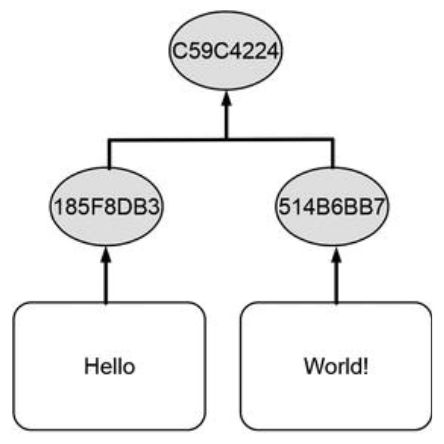
\includegraphics[width=9cm]{img/hashing2}\\[1cm]
\end{center}
\section{Cryptografie}
\textbf{Symmetrische cryptografie}\\*\\*
Bij symmetrische cryptografie bestaat er maar één sleutel voor het encrypteren en het decrypteren. Degene dat het bericht encrypteerde, dus het dus ook terug decrypteren. 
\\*\\*\textbf{Asymmetrische cryptografie}\\*\\*
Asymmetrische cryptografie zit een beetje ingewikkelder in elkaar. Hierbij heb je twee complementaire sleutels. Als een bericht met sleutel A wordt geëncrypteerd, kan dat alleen maar gedecrypteerd worden met sleutel B, zoals getoond in onderstaande foto ~\autocite{blockchain1}. Vandaar de privé sleutel en de publieke sleutel. De privé sleutel is alleen voor de eigenaar die het bericht verstuurd en de publieke sleutel wordt aan iedereen gegeven, zonder te weten of ze betrouwbaar zijn of niet. Merk op dat er dus een bericht kan geëncrypteerd worden met ofwel de privé sleutel of de publieke sleutel, beiden met een verschillende functie. Als een bericht met de privé sleutel geëncrypteerd wordt, kan je dit vergelijken met een broadcast bericht waar iedereen dit kan lezen, want iedereen heeft de publieke sleutel. Als eens bericht met de publieke sleutel geëncrypteerd wordt, dan kan je dit vergelijken met een soort brievenbus. Waar iedereen berichten kan sturen maar alleen de eigenaar ze kan decrypteren.\\*\\*
\begin{center}
	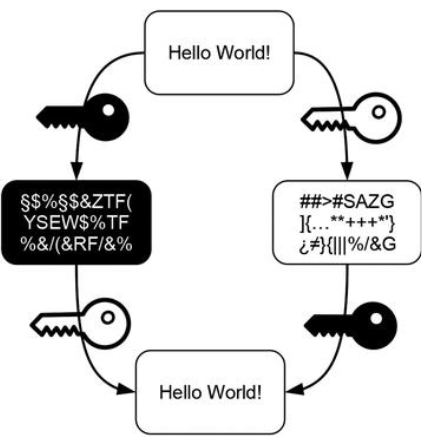
\includegraphics[width=10cm]{img/key}\\[1cm]
\end{center}
\section{Het opslaan van data}
\textbf{De blockchain structuur}\\*\\*
Er werd al eerder uitgelegd dat de structuur van een blockchain vergeleken kan worden met een ketting van blokken. Nu zullen we een beetje dieper ingaan op die structuur. Als er een blok wordt gemaakt met data in, dan wordt deze block gehashed, en deze hash wordt opgeslaan in de header van de volgende blok. Maar hoe ziet de data er precies uit in een blok? De data kan vergeleken worden met een boom structuur. In de kruik staan de transacties, deze worden allemaal gehashed. Daarna worden 2 hash values terug samen gehashed tot op het punt dat er maar 1 hash value aan de wortel van de boom staat. Deze laatste hash value wordt opgeslaan in de header, samen met de hash value van de vorige block.
\\*\\*\textbf{Oude transacties proberen wijzigen}\\*\\*
Daarom is de blockchain dus zo fraudebestendig, omdat alles sequentieel gehashed wordt en zelfs een kleine verandering aan de input een grote verandering kan brengen aan de hash value. Als er iemand de data van transactie 2 wil aanpassen, dan zal de hash value van R2 niet meer kloppen, met het gevolg dat de hash values van R12, B1 en B2 ook niet meer zullen kloppen, zoals getoond in onderstaande foto ~\autocite{blockchain1}. Hierdoor kan de fout heel snel opgespoort worden. Als iemand de informatie in een transactie wil veranderen, dan zal deze persoon elk hash value terug moeten veranderen en dit kost heel veel tijd en computerkracht.\\*\\*
\begin{center}
	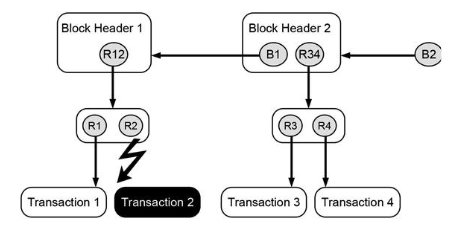
\includegraphics[width=14cm]{img/change}\\[1cm]
\end{center}

\chapter{Supply Chain}
Nu dat we waar bitcoin en blockchain voor staan, is het tijd om te kijken naar supply chain. Wat is een supply chain? Hoe werkt het? Wat loopt er zoal mis?

\section{Wat is een supply chain?}
Een supply chain stelt het fysieke netwerk voor tussen de bedrijven, de leveranciers en de retailers. Het stelt alle stappen voor dat een product ondergaat van begin tot einde. Dit gaat over hoe/waar het product begon als 
rauw material, het transport naar de fabrieken, het proces van de rauwe materialen in de fabriek, distributie over de wereld, transport naar de winkels en zo uiteindelijk naar de klant. Het stelt het hele proces voor.\\*\\* In een supply chain zijn er een paar flows: information flow, product flow, money flow. Information flow vloeit door heen het hele netwerk, van een naar andere peers. Product flow vloeit van de maker naar de eindklant. Money flow vloeit van de eindklant terug naar de maker.\\*\\*Het aspect van betrouwbaarheid binnen een supply chain is heel belangrijk. Er is noodzaak aan vertrouwen van de leveranciers, zodat er geweten is dat je kan rekenen op kwaliteitsvolle producten dat ook optijd geleverd zullen worden. Natuurlijk hebben leveranciers soms ook hun eigen leveranciers, zo worden er al snel meerdere netwerken betrokken bij het op tijd zijn van het proces. Éen fout kan al snel meerdere gevolgen hebben.\\*\\*Het is dus voordelen om de beste oplossing te vinden voor de gekozen supply chain, betere optimalisatie betekent op zijn beurt ook weer mindere kosten en dat betekent minder kosten voor de eindklant. Optimalisatie is key.

\section{Supply Chain Management}
Bij een supply chain, hoort naturlijk ook een supply chain management systeem. Dit is meer te vergelijken met het digitale deel van de supply chain. Supply chain management kan gezien worden als een mantel van activiteiten dat bestaat uit het plannen, controleren en uitvoeren de processen van de supply chain, om dit zo vlot en kost efficiënt mogelijk te maken. Andere taken zijn onder andere controleren en beheren van de inventaris, het regelen van transportatie, het documenteren van alles...\\*\\*Een supply chain kan heel duur en complex zijn, daarom is het belangrijk om zo efficiënt mogelijk te werk te gaan. Er zijn en paar software paketten op de markt dat verspreid gebruikt worden: ERP, Oracle en SAP. Je kan deze software de ruggengraat noemen van een bedrijfscentrische supply chain. Supply chain management zorgt voor de planningen van alle activiteiten, risico beheer, opvolgen en optimaliseren van de inventaris, het regelen van transport, alles documenteren, dag tot dag productie...
~\autocite{scm1}

\chapter{Problemen met supply chain}
Om te weten welke problemen blockchain (niet) kan oplossen voor supply chain, moeten er eerst onderzocht worden welke problemen er precies bestaan. De problemen dat al eerder werden aangehaald in de stand van zaken worden hier kort nog besproken.

\section{Oplossing?}

\begin{enumerate}
	\item \textbf{Globalizering}\\*
		Bedrijven verhuizen bepaalde sectoren naar het buitenland, maar dit brengt meer complexiteit met zich mee. Als deze informatie van de verschillende grafische sectoren nu gecombineerd in één database zou komen, dan wordt dit proces al minder complex. En daar kan blockchain voor zorgen.
	\item \textbf{Vraag en aanbod}\\*
		Het is belangrijk voor de bedrijven dat ze zo snel mogelijk kunnen inspelen op de vraag en aanbod van de eindgebruiker. Via bv. ERP systemen waar de fysieke en digitate supply chain niet altijd gesyncroniseerd zijn, kan dit soms een probleem worden. Bij een blockchain waar er gefocust wordt op snelle transacties, kan deze synchronisatie zo goed als real time zijn.
	\item \textbf{Voldoen aan de verwachtingen van de eindgebruiker}\\*
		De eindgebruiker verwacht dat de producten dat gekocht worden, altijd van goeie kwaliteit zijn. Alhoewel blockchain hierop een indirecte relatie kan uitoefenen via het naar omlaag brengen van de kosten, is er geen directe relatie tussen het gebruik van blockchain en de kwaliteit van de producten.
	\item \textbf{Veel papier werk}\\*
		Dit is een punt dat zeker kan opgelost worden via blockchain. Omdat meerdere bedrijven dezelfde informatie moet invullen, is er meer plaats voor fouten te maken. Deze informatie is ook redundant omdat elk bedrijf dit zelf wil bijhouden omdat er geen vertrouwen is tussen de verschillende partijen. Dit is dus perfect voor blockchain, omdat blockchain het vertrouwensprobleem oplost. Documenten kunnen ook worden opgeslaan op de blockchain, zodat deze veel makkelijker toegankelijk zijn voor de correcte lezer ervan.
	\item \textbf{Wat nu voor de lokale chinese boeren?}\\*
		Omdat deze boeren nog hevig gecontroleerd, getakseerd en gemanipuleerd worden, is het moeilijk van in te stappen in blockchain. Deze boeren hebben meestal ook de middelen er niet voor. Blockchain kan voor hun ook niets veranderen aan de kwaliteit van de producten, de slechte wegen en het landschap. Terwijl het voor grotere bedrijven wel een mogelijkheid is.
\end{enumerate}

\section{Conclusie problemen}
De vraag 'Welke problemen kunnen niet opgelost worden met blockchain?' kan nu al beantwoord worden met de met de informatie dat er tot nu toe al verzameld is in dit hoofdstuk. Terwijl blockchain redelijk wat problemen kan oplossen voor supply chain, zijn er ook een antal dat hier onderzocht werden, waar blockchain een mindere betekenis heeft. Blockchain kan op zich niet direct iets veranderen aan de kwaliteit van de producten, deze verantwoordelijkheid ligt nog altijd bij het bedrijf zelf. Ook is het moeilijk voor de lokale boeren dat niet de middelen hebben om te starten met de integratie met blockchain. Als er gekeken wordt naar China, zijn daar de omstandigheden ook heel moeilijk.

\chapter{HyperLedger composer prototype}
\section{Wat is hyperledger composer?}
Hyperledger composer is een open ontwikkelings tool om blochchain applicaties te maken. Een business netwerk kan makkelijk worden omgezet in een blockchain netwerk. Het maakt gebruik van middelen, zoals tomaten, certificaten, vervoer. Het maakt gebruik van transacties dat inwerkt in de middelen. Daarnaast heb je ook nog toegang tot toeganscontrole, identiteiten en andere deelnemers in het netwerk, zoals de koper en verkoper, leveranciers en fabrieken.\\*\\*Met hyperledger composer kan een protoype opgezet worden om de supply chain te simuleren in de agricultuur.
~\autocite{composer1}

\section{Netwerk voorstelling}
Om deze simulatie zo goed mogelijk te laten verlopen, werd er een fictief netwerk opgesteld van bedrijven. Deze bedrijven bevatten de volgende soorten: "supplier", "manufacturer", "contributer", "retailer", "customer". Elk soort bedrijf heeft een paar voorbeelden gekregen. Buiten de bedrijven mogen we de producten ook zeker niet vergeten. In dit netwerk draait alles om tomaten. Wat er nodig is om tomaten te maken, van deze tomaten producten maken en deze te verkopen. Naast de bedrijven en producten, hebben alle bedrijven ook een eigen Wallet, voor de transacties zo goed mogelijk te simuleren. Hier onder wordt er een tabel gegeven van alle informatie dat beschikbaar is:

Zie Bijlage C voor alle gegevens te bekijken.

Een netwerk in supply chain is nooit zomaar een ketting van bedrijven. Het is een heel netwerk op zich. De ene output van een bedrijf kan de input betekenen van een ander bedrijf. Een bedrijf heeft veel verschillende zaken nog voor het maken van een product, maar in deze simulatie wordt er gefocust op tomaten. Zie hier een foto van 1 ketting in een heel netwerk:

\begin{center}
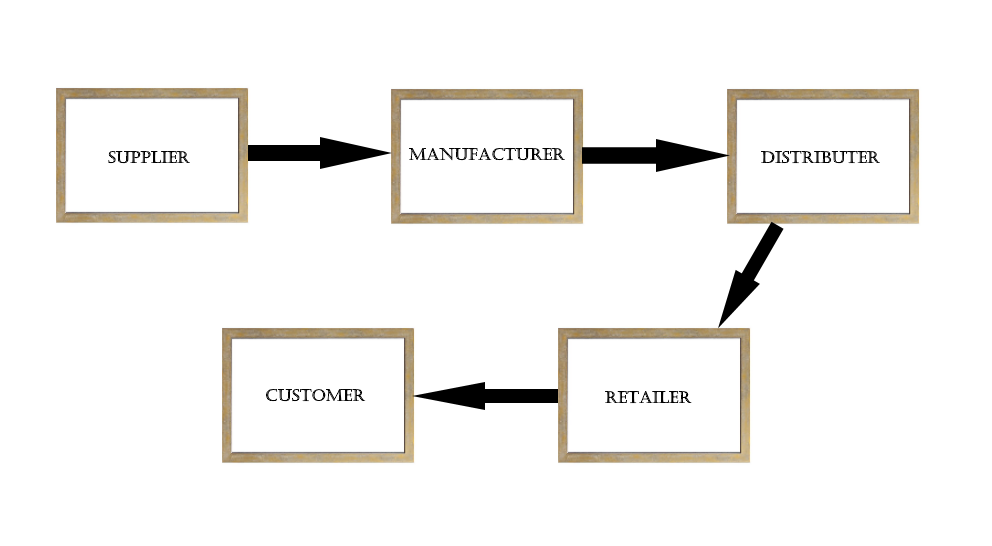
\includegraphics[width=15cm]{img/ketting}\\[2cm]
\end{center}

Maar meestal is een supply chain netwerk niet gewoon 1 ketting, maar dan bestaat dit uit een netwerk van kettingen, zoals dit te zien is op onderstaande foto ~\autocite{pic1}.

\begin{center}
	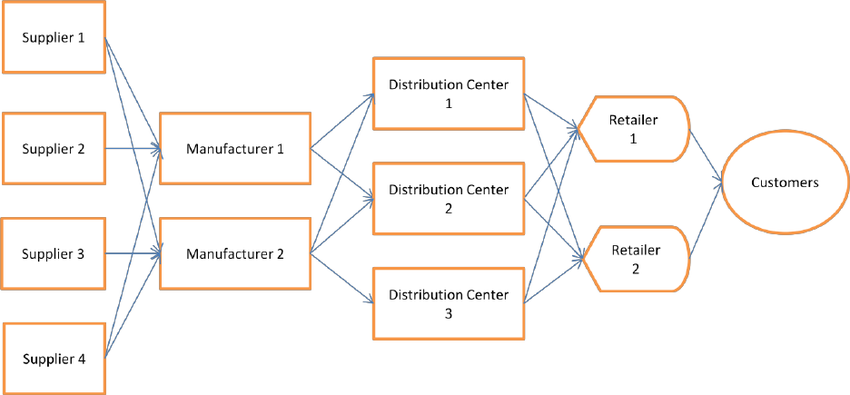
\includegraphics[width=15cm]{img/netwerk}\\[3cm]
\end{center}
\section{Gebruikte technologieën}
\textbf{HyperLedger Composer}

Met behulp van de HyperLedger composer, is er een netwerk opgesteld van bedrijven en producten. De volgende 3 foto's beschijven de stappen van het starten van het netwerk.
Hiervoor zijn een paar stappen nodig:

\begin{enumerate}
	\item Hyperledger fabric starten starten
	\begin{center}
		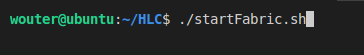
\includegraphics[width=8cm]{img/start-fabric}\\[1cm]
	\end{center}
	Om het netwerk te gebruiken en er moeten we het eerste starten met bovenstaande starten. In dit voorbeeld is hyperledger fabric al geïnstalleerd.\\*
	\item Netwerk starten
	\begin{center}
		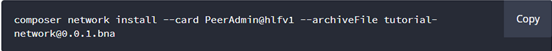
\includegraphics[width=13cm]{img/install-network}\\[1cm]
		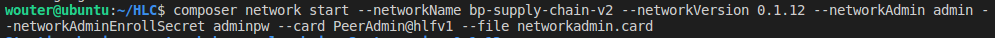
\includegraphics[width=14cm]{img/start-network}\\[1cm]
	\end{center}
	Bij het installeren en het starten van het netwerk worden gegevens meegegeven zoals de admin kaart, de bna file waar alles gecompesseerd instaat, de versie van het netwerk dat ingesteld wordt in de package.json...\\*
	\item Composer rest server starten
	\begin{center}
		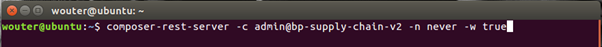
\includegraphics[width=13cm]{img/start-rest}\\[1cm]
	\end{center}
	Via HyperLedger wordt er gezorgd voor een rest-api server. Met behulp van deze lokale server kunnen er verzoeken verzonden worden vanaf een applicatie naar de rest-api server dat op zich de nodige data uit het netwerk zal halen. Hier wordt meer op in gegaan in het deel van NodeJS.\\*
\end{enumerate}

Het netwerk bestaat uit een aantal bestanden: een model bestand, waar alle bedrijven en producten worden gedefiniëerd, maar ook de verschillende transacties. Een logica bestand waar de logica instaat tijdens het uitvoeren van een transactie. Er wordt ook gebruik gemaakt van een acces file, hierin staan alle beveiligingsregels van wie wat mag doen op het netwerk. Er wordt niet verder ingegaan op dit bestand in deze simulatie.

Dit is de gebruikte structuur van het model bestand. Op de foto is onder andere het product en het bedrijf te zien, net zoals een transactie en een event declaratie.\\*\\*In de volgende foto is dan weer de logica te zien van een transactie. Hier in wordt het register van alle producten opgehaald en wordt het product dat aangepast wordt geüpdatet. Daarna wordt er een nieuwe event aangemaakt dat zichtbaar zal zijn in de NodeJS applicatie.

\begin{center}
	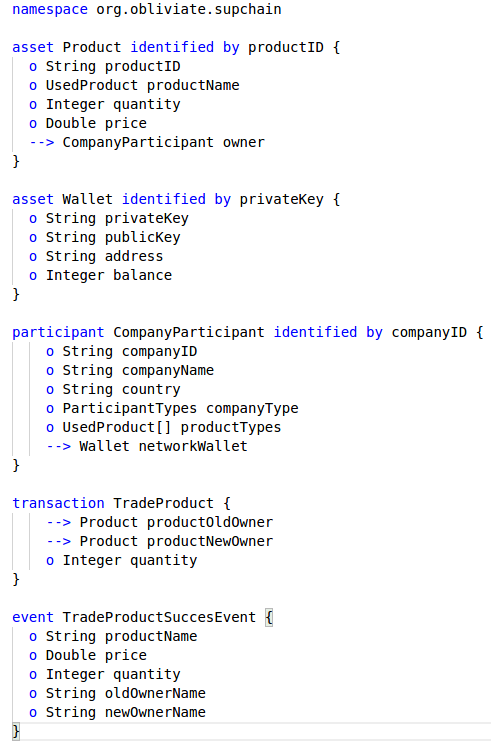
\includegraphics[width=11cm]{img/model-example}\\[1cm]
\end{center}

\begin{center}
	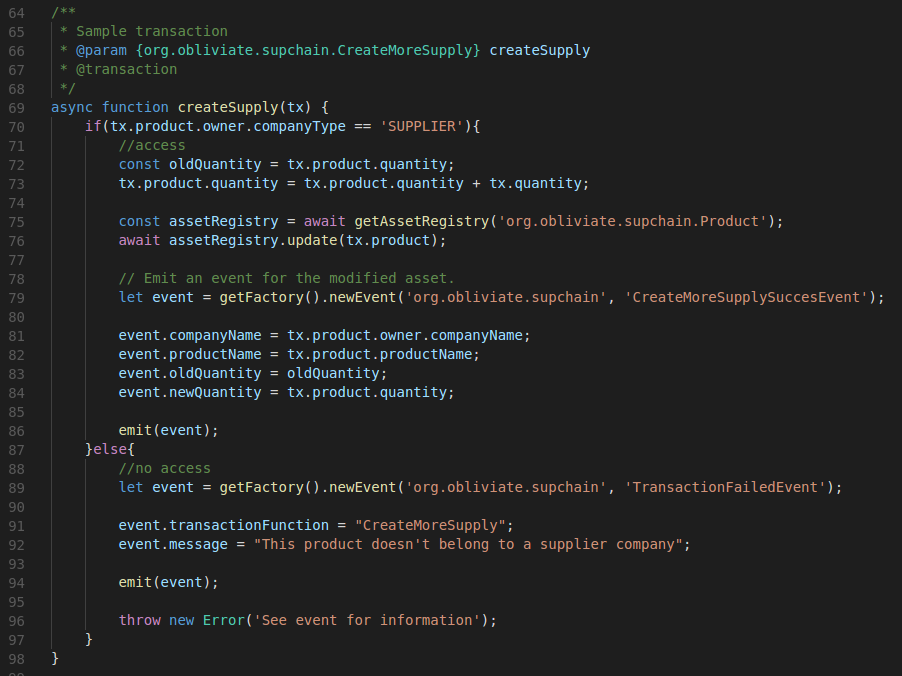
\includegraphics[width=14cm]{img/logic-example}\\[1cm]
\end{center}

\textbf{NodeJS}

Omdat het netwerk elk keer weer leeg is als het opnieuw wordt opgestart, moeten we een manier vinden het netwerk terug te vullen met informatie. Dit kan gedaan worden door de "composer-client" package te gebruiken in NodeJS.

Eerst zal er een connectie gemaakt moeten worden met het netwerk via de "composer-client":
\begin{center}
	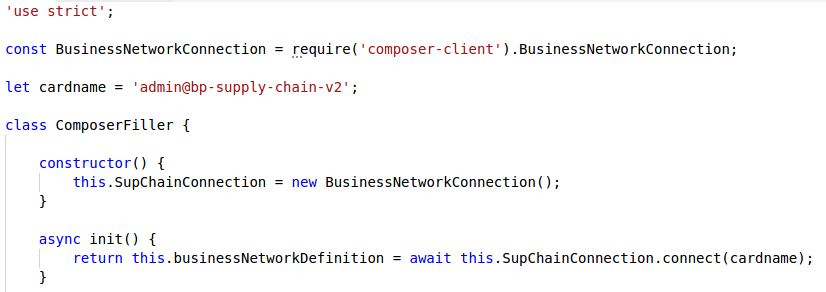
\includegraphics[width=13cm]{img/composer-start}\\[1cm]
	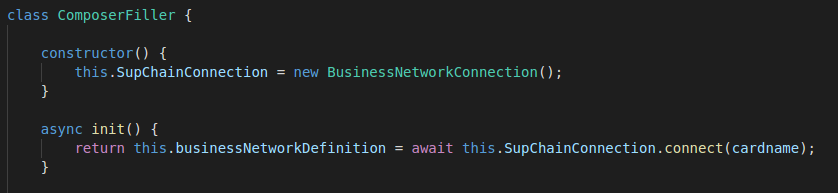
\includegraphics[width=13cm]{img/composer-connect}\\[1cm]
\end{center}

Er zijn 3 verschillende scripts geschreven: een script om het netwerk te vullen met gegevens, een script om alle informatie in het netwerk te verwijderen en een script dat luistert naar event uit het netwerk.\\*

\begin{center}
	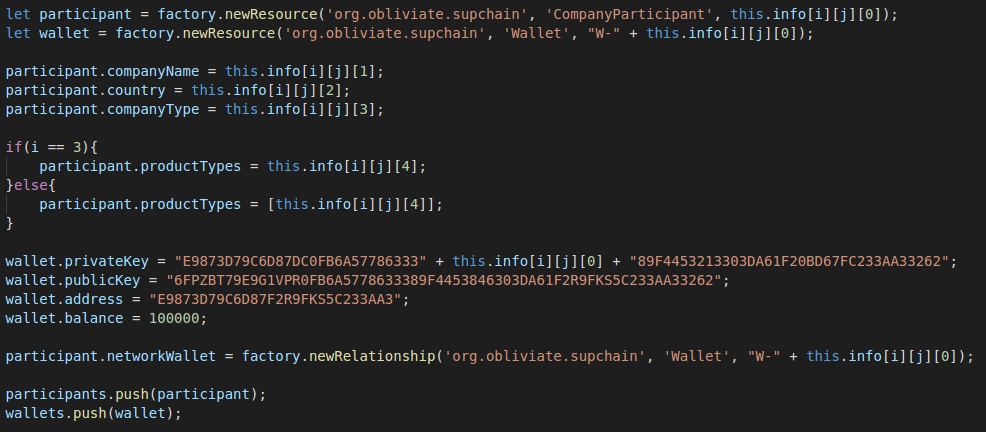
\includegraphics[width=14cm]{img/create-create}\\[1cm]
	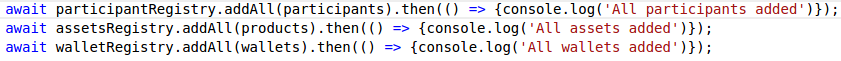
\includegraphics[width=14cm]{img/create-send}\\[1cm]
\end{center}

In het script om het netwerk met gegevens te vullen, wordt er van elk gegeven het bijhorende object gemaakt, dit wordt gepushed in een overkoepelende array en dan in één keer naar het netwerk verstuurd.

\begin{center}
	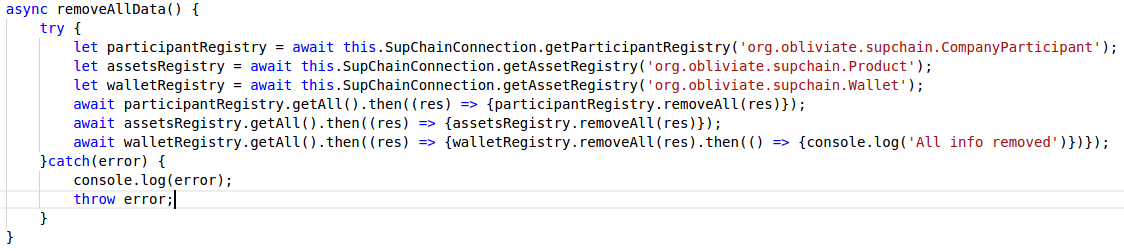
\includegraphics[width=14cm]{img/delete-delete}\\[1cm]
\end{center}

In het script om alle informatie te verwijderen, wordt eerst alle informatie opgehaald met de registers en daarna allemaal verwijderd.

\begin{center}
	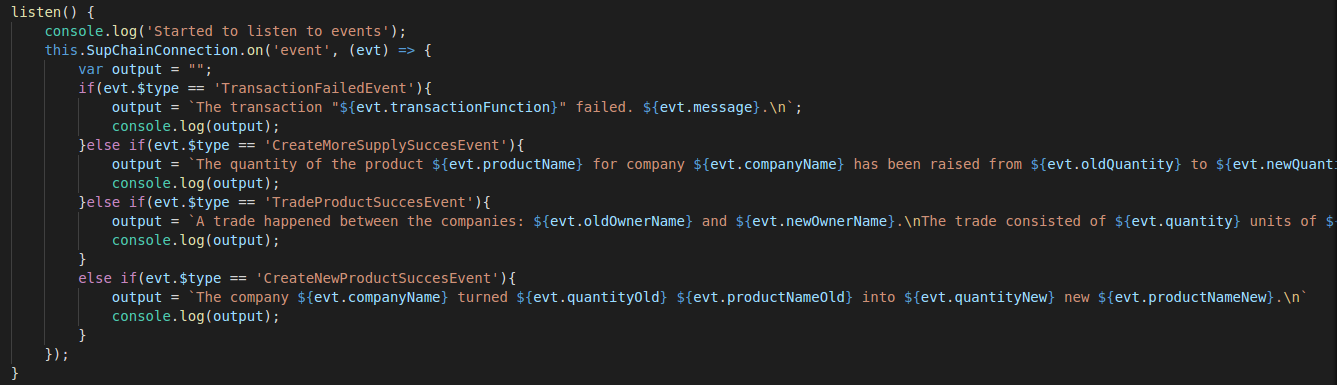
\includegraphics[width=14cm]{img/listen-listen}\\[1cm]
\end{center}

In het script dat luistert naar de verschillende events, wordt er elke keer dat er een event ontvangen wordt naar de naam gekeken en gebaseerd daarop wordt de juiste melding terug gegeven.

\begin{center}
	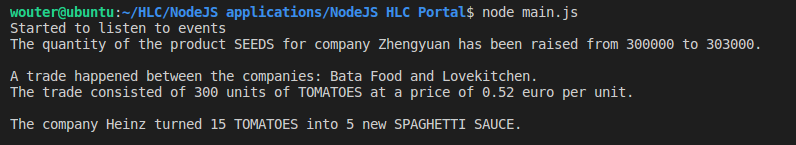
\includegraphics[width=14cm]{img/listen-results}\\[1cm]
\end{center}

\textbf{React Native}

Als voorbeeld werd er een mobiele applicatie geschreven.Later in de demonstratie wordt hier grondiger op in gegaan. In deze applicatie heeft de gebruiker de keuze tussen de soorten bedrijven en daarna een specifiek bedrijf binnen die branche. De gebruiker krijgt de keuze tussen 3 acties dat een bedrijf kan verrichten, van zodra de correcte gegevens worden ingevuld, krijgt de gebruiker een overzicht te zien van alle specifieke stappen dat ondergaan werden tijdens de transactie. Hieronder volgen nog een paar voorbeelden van gebruikte code:

\begin{center}
	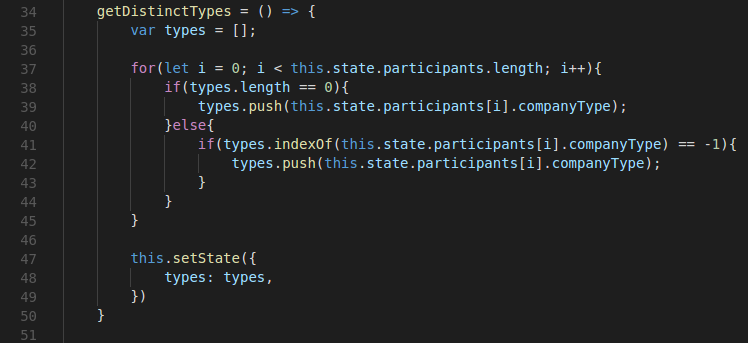
\includegraphics[width=14cm]{img/react-types}\\[1cm]
\end{center}

In de bovenstaande foto wordt er naar elk type gekeken van elk bedrijf. Alleen als dat type nog niet in de array staat, wordt deze toegevoegd. Dit is belangrijk om dynamisch alle soorten bedrijven op te halen.

\begin{center}
	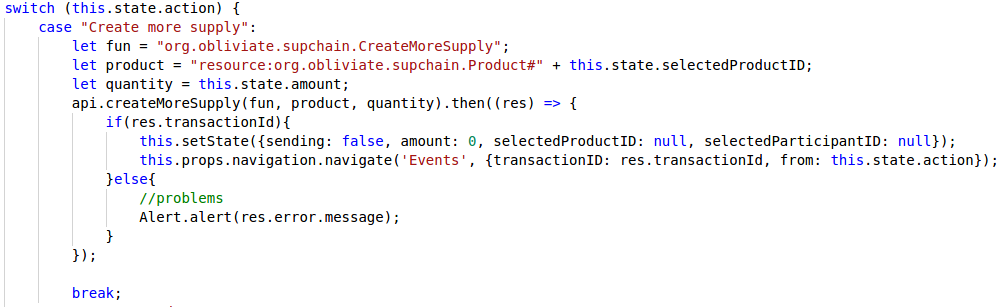
\includegraphics[width=14cm]{img/react-action}\\[1cm]
\end{center}

Dit is een voorbeeld van een transactie verzonden wordt vanuit de front-end. Het is nodig om de juiste transactienaam mee te geven, samen met de bijhorende variabelen zoals het product en het aantal.

\begin{center}
	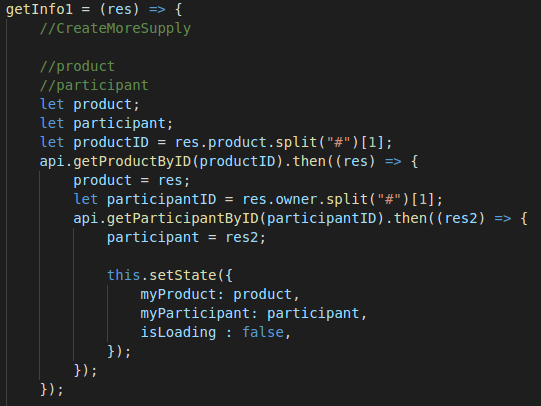
\includegraphics[width=14cm]{img/react-info}\\[1cm]
\end{center}

Elke transactie op het netwerk heeft zijn eigen transactieID. Dit kregen we terug in de vorige foto. Met dit transactionID kunnen we de volledige transactie terug ophalen en daar de gegevens ook terug uithalen.

\begin{center}
	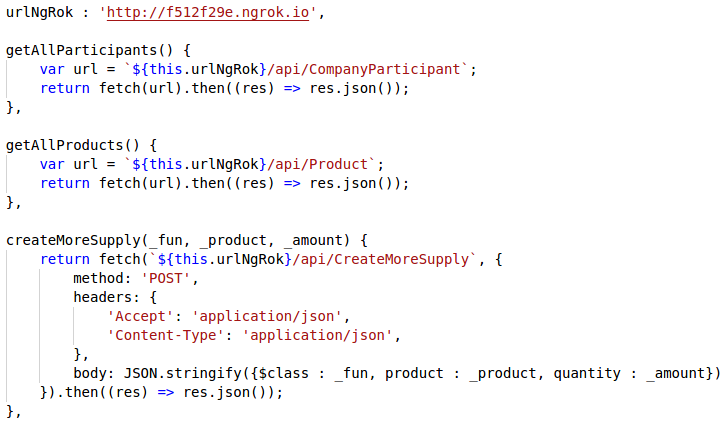
\includegraphics[width=14cm]{img/react-api}\\[1cm]
\end{center}

Om dit alles te kunnen doen, moet er natuurlijk een api worden aangesproken. Omdat de API normaal op een localhost draait, gebruiken we NgRok om dit open te stellen op het internet. Daarna kan je de correcte link aanroepen en ofwel een get, post, delete, put verzoek sturen naar de server.

\section{Demonstratie}

\textbf{Demonstratie 1}

Zie Bijlage A waar de screenshots staan van de applicatie. Deze screenshots zijn per demonstratie in de juiste volgorde gezet.

Bij het openen van de applicatie wordt de keuze gegeven tussen de verschillende soorten bedrijven, in het eerste voorbeeld wordt de "SUPPLIER" genomen. Daarna komt er een nieuw scherm waar de keuze gemaakt wordt tussen de verschillende bedrijven.

Elk soort bedrijf heeft zijn eigen acties dat ze kunnen uitvoeren op het netwerk. Een supplier kan nu alleen maar zijn eigen voorraad vergroten. Bij het uitvoeren van de actie wordt er gevraagd naar het bepaalde product en hoeveelheid. De getoonde producten in de lijst zijn alleen maar producten dat dat ene bedrijf kan maken.

In de laatste stap van de applicatie wordt er stap voor stap getoond wat er precies allemaal gebeurt tijdens de transactie. Er wordt informatie getoond zoals de naam van het bedrijf en de voorraad van het bepaalde product.


\textbf{Demonstratie 2}

De uitleg bij demo 2 en 3 zijn grotendeels hetzelfde. De flow van de applicatie is makkelijk af te leiden ui de screenshots.

Zie Bijlage A demo 2.

\textbf{Demonstratie 3}

Zie Bijlage A demo 3.

\section{Mogelijke uitbreidingen}
Natuurlijk is dit nog maar een minimaal prototype, er zijn zeker nog veel mogelijke uitbreidingen.\\*\\*
Een van de belangrijkste uitbreidingen dat hier nog gemaakt kunnen worden is het implementeren van een zoekfunctie dat voor de gebruiker een perfecte route gaat zoeken. Er zou dan gefilterd kunnen worden op snelste route, goedkoopste route, de route met de beste kwaliteit of combinatie van meerdere factoren. Omdat de prijzen van de bedrijven openlijk verkrijgbaar zijn op het netwerk, is deze optie zeker doenbaar.\\*\\*Een logische uitbreiding is het toevoegen van meerdere producten in de supply chain. Zoals voor de bedrijven dat lasagne of soep maken, zullen er meer producten nodig zijn dan alleen maar tomaten. Dit geldt natuurlijk ook voor meerdere bedrijven.\\*\\*In dit prototype is niet verder ingegaan op de access file, dat kan ook een verdere uitbreiding worden. Dankzij de access file wordt er beslist wie precies wat mag doen op het netwerk.

\section{Conclusie Hyperledger composer}
De vraag 'Hoe kan er met zekerheid gezegd worden dat de producten authentiek zijn?' kan nu al beantwoord worden met de met de informatie dat er tot nu toe al verzameld is. Op de manier dat informatie wordt opgeslagen op een blockchain kan er gezegd worden dat deze informatie niet aangepast kan worden, de data kan niet vervalst worden. Als een persoon deze informatie wil veranderen, zal de hash waarde niet meer overeenkomen met de historiek van andere nodes. Deze persoon zou daarom alle hash waarden moeten gaan aanpassen, en dat is nu onmogelijk. Op het netwerken heeft een bedrijf ook bepaalde rechten, dus een bedrijf kan niet zo maar de voorraad van een ander bedrijf gaan aanpassen. Dankzij deze historiek dat bijgehouden wordt kan er perfect aangetoond worden van waar een product precies afkomstig is en kan deze informatie dus ook als betrouwbaar aanzien worden.

\chapter{Uitvoeren testen}
\section{Schetsen van de situatie}
Voor een bedrijf is de snelheid van het netwerk ook zeker een belangrijk aspect. Een bedrijf kan niet zitten wachten op transacties dat in queue staan om uitgevoerd te worden. Daarom worden er ook een paar snelheidstesten losgelaten op het netwerk. Dit netwerk werd opgesteld op een virtuele machine, de testen duren daarom dus ook langer dan normaal. Op volgende transacties wordt de snelheid getest:\\*
\begin{enumerate}
	\item Creatie van informatie
	\item Verwijderen van informatie
	\item Ophalen van alle producten / bedrijven
	\item Opzoeken van één bepaalde ID
\end{enumerate}

\section{Uitgevoerde testen}
Elke test wordt 30 keer uitgevoerd...\\*\\*
\textbf{Creatie van informatie}

Er worden twee verschillende testen uitgevoerd voor de creatie van de informatie. De gegevens kunnen in één lijst verstuurd worden om aan te maken op het netwerk of dit kan gegeven per gegeven verstuurd worden. Hier wordt getest of er een verschil bestaat tussen deze twee manieren. Er werd getest met 5, 50 en 100 producten. Er worden geen testen uitgevoerd met meer producten omdat er vanaf dan timeout errors worden gegeven.

\begin{center}
	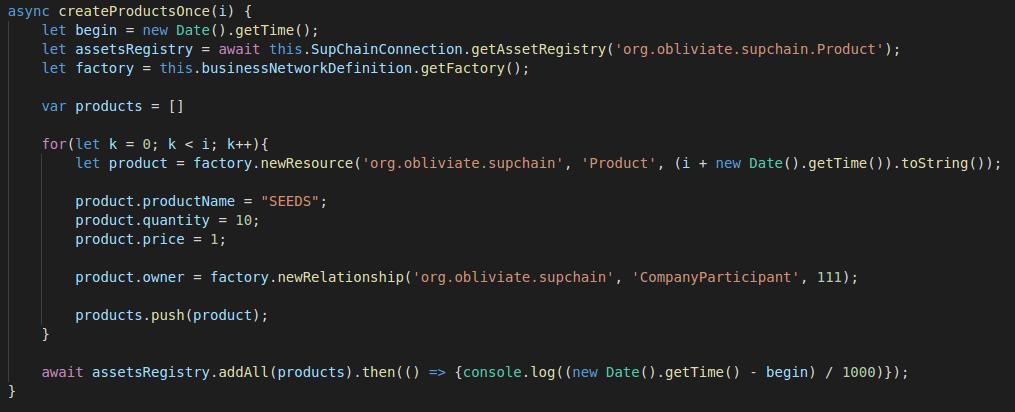
\includegraphics[width=14cm]{img/test-function-createProductOnce}\\[1cm]
\end{center}

\textbf{Verwijderen van informatie}

De volgende transactie dat getest zal worden is het verwijderen van alle informatie. Dit kan ook gebeuren één per één of alles in één keer. Hierbij wordt er ook getest met 5, 50 en 100 producten.

\begin{center}
	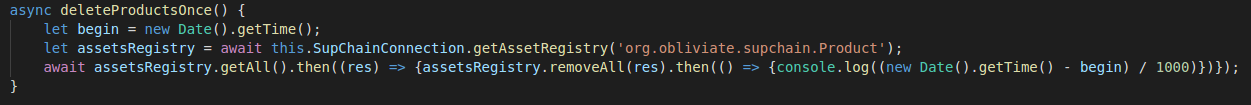
\includegraphics[width=14cm]{img/test-function-removeProductOnce}\\[1cm]
\end{center}

\textbf{Ophalen van alle producten / bedrijven}

Bij deze test is het de bedoeling om te kijken of er een groot verschil bestaat tussen het opvragen van alle informatie. Hier wordt er nogmaals gebruik gemaakt van 5, 50 en 100 producten.

\begin{center}
	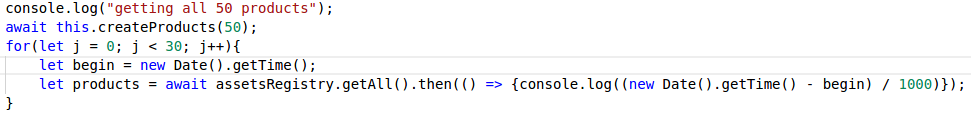
\includegraphics[width=14cm]{img/test-function-getAllProducts}\\[1cm]
\end{center}

\textbf{Opzoeken van één bepaalde ID}

Als laatste wordt er onderzocht of er een verschil bestaat tussen het ophalen van één bepaald product in een lijst van meerdere producten. Nogmaals worden er hier 5, 50 en 100 producten gebruikt.

\begin{center}
	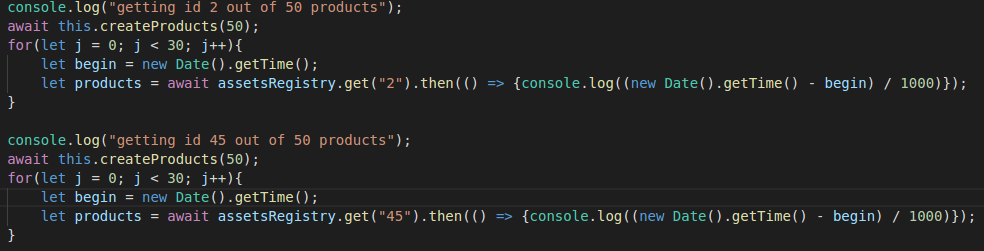
\includegraphics[width=14cm]{img/test-function-getID}\\[1cm]
\end{center}

\section{resultaten}
Alle resultaten zijn uitgedrukt in seconden...
\begin{enumerate}
	\item Creatie van informatie\\*
	
		\textbf{Alle producten in 1 keer}\\*
		
		 Voor de ruwe resultaten, zie Bijlage B.\\*
		
		\textbf{Alle producten apart}\\*
		
		 Voor de ruwe resultaten, zie Bijlage B.\\*
		
		\begin{center}
			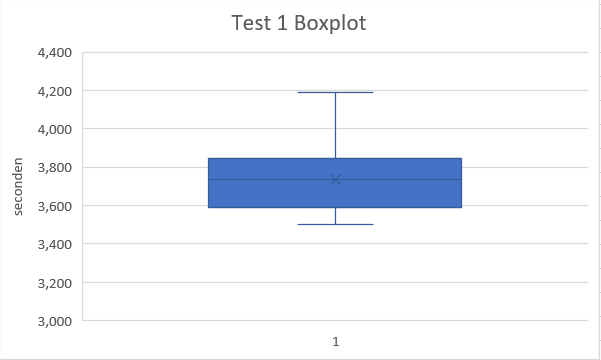
\includegraphics[width=12cm]{img/test-box-1}\\[1cm]
		\end{center}\begin{center}
			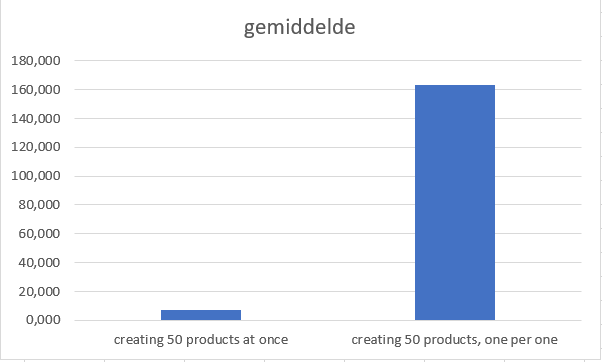
\includegraphics[width=12cm]{img/test-column-1}\\[1cm]
		\end{center}
		Als er gekeken wordt naar het gemiddelde van 50 producten in één keer toevoegen of 50 producten één voor één toevoegen, kan er geconcludeerd worden dat er toch een redelijk groot verschil bestaat tussen deze twee manieren. Er wordt elke keer een extra call gedaan naar het netwerk en daar wordt er tijd verloren. Voor het apart toevoegen van 50 prodcuten kan het wel tot bijna 3 minuten duren.\\*
		
		
	\item Verwijderen van informatie\\*
	
		 Voor de ruwe resultaten, zie Bijlage B.\\*
		
		\begin{center}
			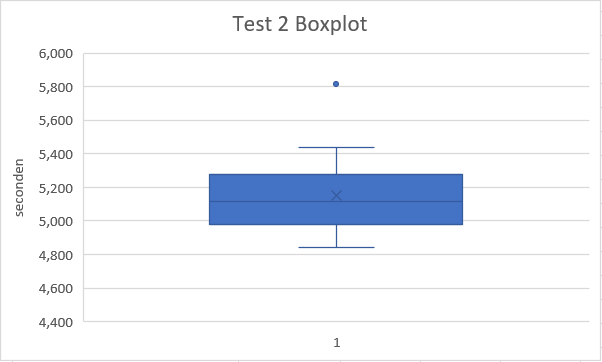
\includegraphics[width=12cm]{img/test-box-2}\\[1cm]
		\end{center}\begin{center}
			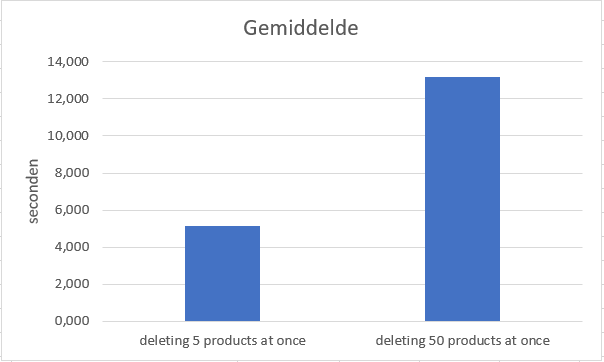
\includegraphics[width=12cm]{img/test-column-2}\\[1cm]
		\end{center}
		Bij het verwijderen van gegevens konden de testen van het product een voor een te verwijderen niet uitgevoerd worden. Omdat deze veel te lang duurde gaf het netwerk een time out. De tijd bij deze testen is langer dan verwacht, het verwijderen duurt langer dan het aanmaken. Opnieuw liggen de resultaten dicht bij elkaar.\\*
	
	\item Ophalen van alle producten / bedrijven\\*

		 Voor de ruwe resultaten, zie Bijlage B.\\*

		\begin{center}
			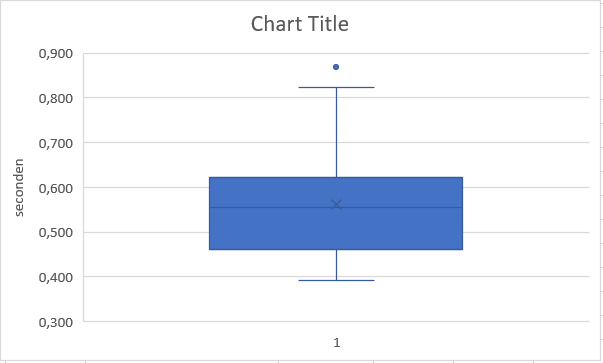
\includegraphics[width=12cm]{img/test-box-3}\\[1cm]
		\end{center}\begin{center}
			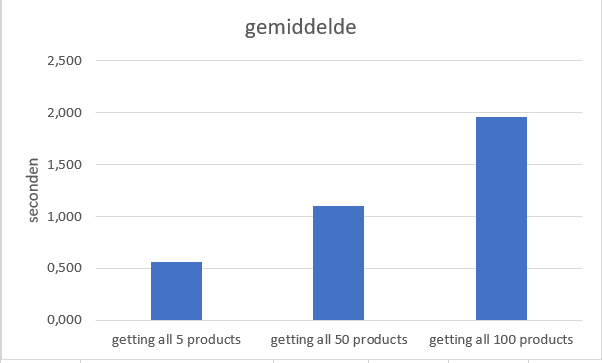
\includegraphics[width=12cm]{img/test-column-3}\\[1cm]
		\end{center}
		In deze liggen de resultaten een beetje meer verspreid van elkaar als er gekeken wordt naar de boxplot. Het ophalen van alle gegevens gaat nog relatief gezien snel in vergelijking met het toevoegen en verwijderen.\\*
	
	\item Opzoeken van één bepaalde ID\\*
	
		 Voor de ruwe resultaten, zie Bijlage B.\\*
	
		\begin{center}
			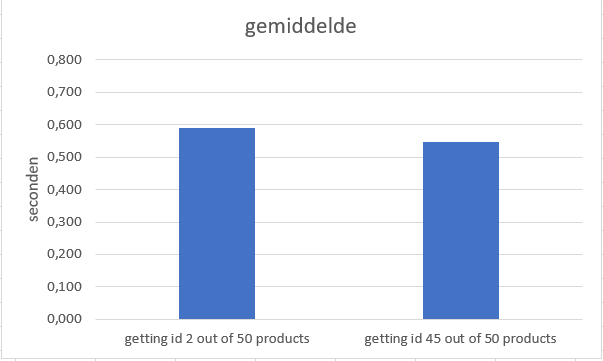
\includegraphics[width=11cm]{img/test-column-4}\\[1cm]
		\end{center}
		\begin{center}
			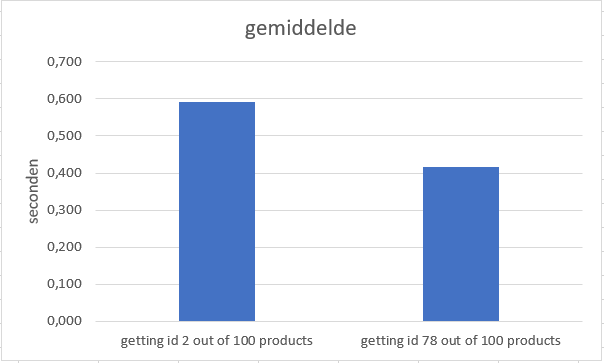
\includegraphics[width=11cm]{img/test-column-5}\\[1cm]
		\end{center}
		Wat heel merkwaardig is bij deze testen is dat het blijkt dat de producten met de hogere id's minder lang duren dan de producten met een klein id. Dit kan zijn omdat de lijst omgekeerd onderzocht wordt, maar hier werd niet meer informatie over gevonden.
\end{enumerate}
\section{conslusie resultaten}
Spijtig genoeg konden sommige testen niet worden uitgevoerd omdat het netwerk te traag was op de virtuele machine. De conclusie uit deze testen is dat het altijd beter is om een hele lijst mee te geven aan een functie dan elk object apart te versturen.De resultaten zijn redelijk consistent in de uitvoeringstijd als er gekeken wordt naar de boxplotten. Soms waren er verassende resultaten zoals het verwijderen dat langen duurt dan het toevoegen en het ophalen van een hoger id dat minder lang duurde dan het ophalen van een lager id.

\chapter{Toekomstig werk}
Zoals eerder al aangehaald in deze bachelorproef, blijft technologie maar evolueren. Het is belangijk dat er mee wordt gegaan met de tijd. Blockchain technologie staat nog in zijn peuterschoentjes en er is nog veel dat onderzocht moet worden in verband met decentralisatie, beveiliging en uitbreidbaarheid. Het hele gebeuren rond supply chain is ook heel complex, er zal diep onderzoek gedaan moet worden hoe deze twee technologieën perfect in harmonie kunnen samenwerken. Bijvoorbeeld kan er een meer dynamisch netwerk opgesteld worden waardat de gebruikers zich werkelijk inloggen als een bedrijf en zelf ook producten kunnen toevoegen en bij andere bedrijven verkopen en kopen.\\*\\*
Wat nog verder getest kan worden is de transparantie van het netwerk. Wat mag een bedrijf bekijken op het netwerk en wat niet. Kiest een bedrijf er zelf voor of het zichtbaar is naar de buitenwereld enzovoort.\\*\\*
Deze bachelorproef creëert ook nog een paar andere vragen wat verder onderzocht moet worden:

\begin{enumerate}
	\item Voor welke bedrijven is het nuttig om met blockchain technologie te integreren?
	\item Wat is nuttiger voor een supply chain netwerk? Publiek of privaat?
	\item Welke blockchain technologie kan het beste gebruikt worden voor een supply chain?
\end{enumerate}

%%=============================================================================
%% Conclusie
%%=============================================================================

\chapter{Conclusie}
\label{ch:conclusie}

De onderzoeksvragen worden snel nog eens hieronder geplaatst:
\begin{enumerate}
	\item \textbf{Hoe kan er met zekerheid gezegd worden dat de producten authentiek zijn?}\\*
	\item \textbf{Heeft het aantal gegevens op het netwerk een invloed op het ophalen en wegsturen van informatie?}\\*
	\item \textbf{Welke problemen kunnen (nog) niet opgelost worden met blockchain?}\\*
\end{enumerate}

In de conclusie worden de onderzoeksvragen nog eens overlopen en wordt er hier een antwoord op gegeven.\\*\\*
Dankzij de blockchain technologie kunnen we met zekerheid zeggen dat de authentiteit van producten behouden wordt. Eens de informatie op de blockchain staat, kan die transactie niet meer aangepast worden. Op het netwerk heeft alleen de eigenaar rechten tot zijn producten en kiest dus zelf wat er met gebeurt. Hierdoor kunnen andere bedrijven geen producten gaan aanpassen van andere bedrijven. Dankzij de historiek van de blockchain kan er gezien worden wat er exact met elk product gebeurt, en zo kunnen de eindgebruikers dus ook met zekerheid zien waar hun prouct precies vandaag komt.\\*\\*
Het aantal gegevens heeft dus duidelijk wel een invloed op de snelheid van het ophalen en wegschrijven van informatie. Uit de resultaten kan er afgeleid worden dat het effeciënter wordt als er een grotere lijst wordt ingevoerd. Spijtig genoeg zijn sommige testen niet kunnen doorgaan door het te kort komen van de virtuele machine waarop het netwerk draaide.\\*\\*
Ten slotte werd er gekeken naar wat een blockchain (nog) niet kan oplossen als blockchain gecombineerd wordt met supply chain. Blockchain kan op zich niet direct iets veranderen aan de kwaliteit van de producten, deze verantwoordelijkheid ligt nog altijd bij het bedrijf zelf. Ook is het moeilijk voor de lokale boeren dat niet de middelen hebben om te starten met de integratie met blockchain. Als er gekeken wordt naar China, zijn daar de omstandigheden ook heel moeilijk. 


%%=============================================================================
%% Bijlagen
%%=============================================================================

\appendix

%%---------- Onderzoeksvoorstel -----------------------------------------------

\chapter{Onderzoeksvoorstel}

Het onderwerp van deze bachelorproef is gebaseerd op een onderzoeksvoorstel dat vooraf werd beoordeeld door de promotor. Dat voorstel is opgenomen in deze bijlage. Door veranderingen na het voorstel is dit voostel niet helemaal up to date. Dit voorstel moest dus ook niet aangepast worden voor deze bachelorproef.

% Verwijzing naar het bestand met de inhoud van het onderzoeksvoorstel
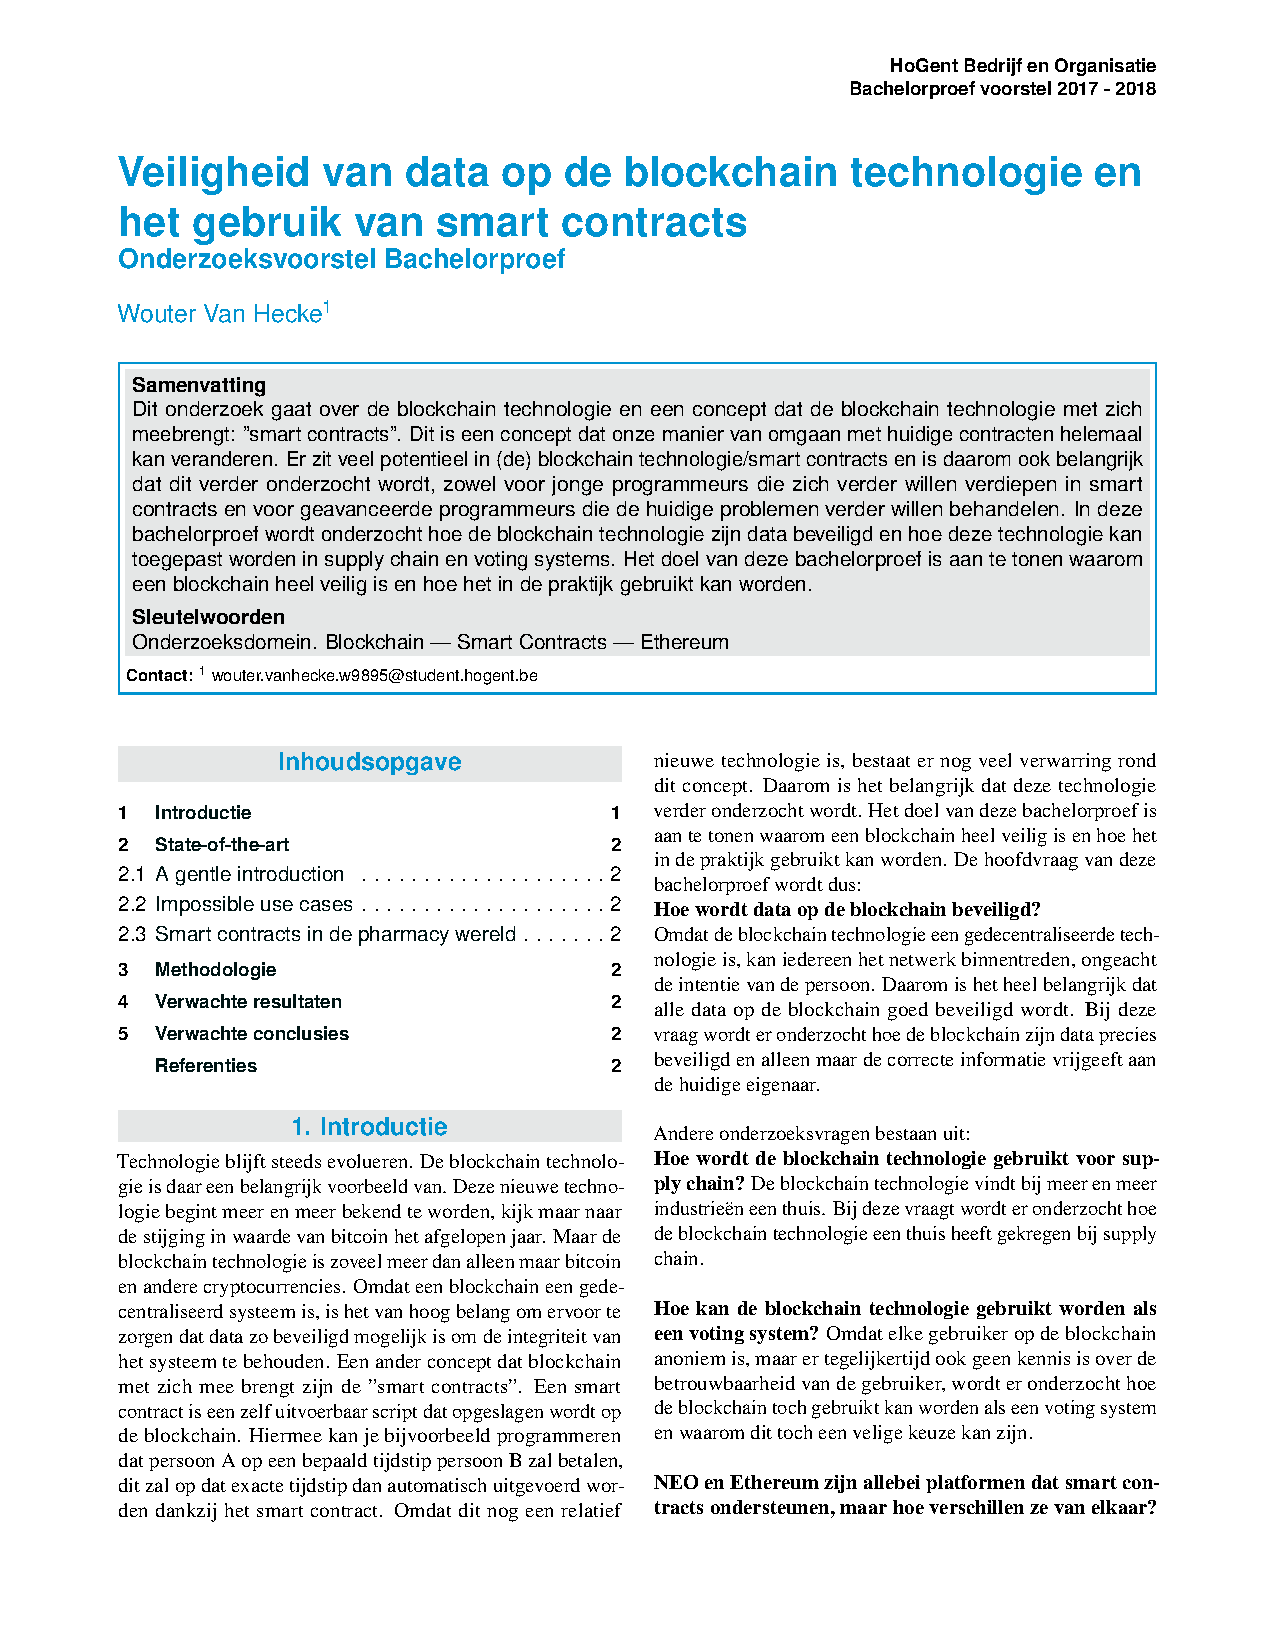
\includepdf[pages=-]{../voorstel/vanhecke_wouter_voorstel.pdf}

%%---------- Andere bijlagen --------------------------------------------------
% TODO: Voeg hier eventuele andere bijlagen toe
\chapter{Bijlage}
\section{Demonstratie applicatie}
\textbf{Demonstratie 1}
\begin{center}
	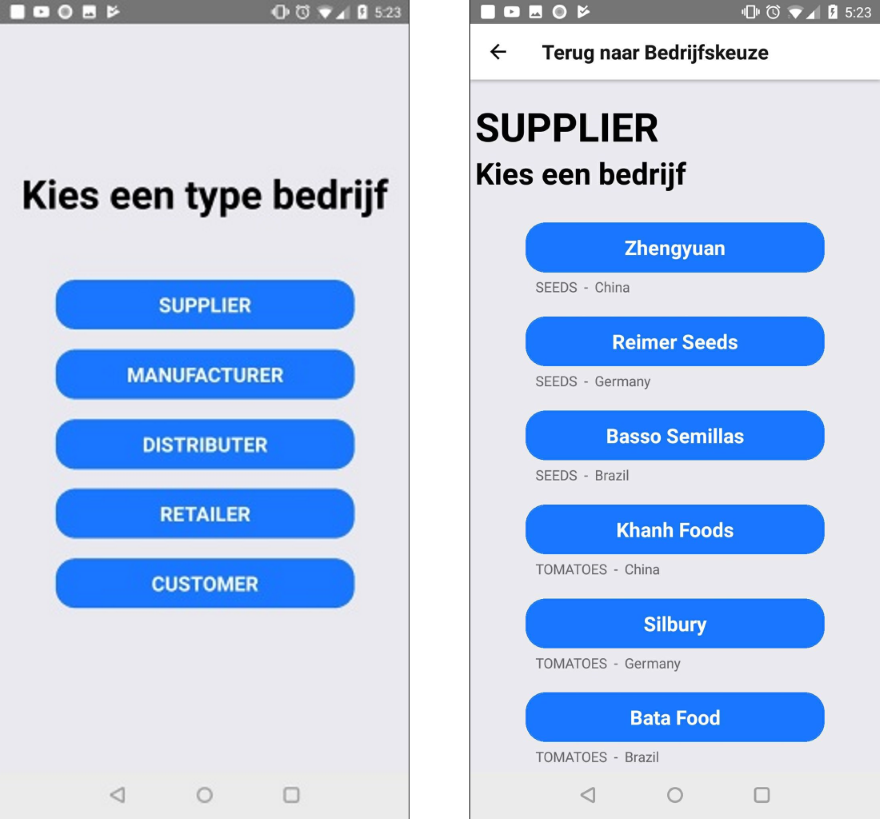
\includegraphics[width=11cm]{img/react-demo-1-1}\\[1cm]
	...
\end{center}

\begin{center}
	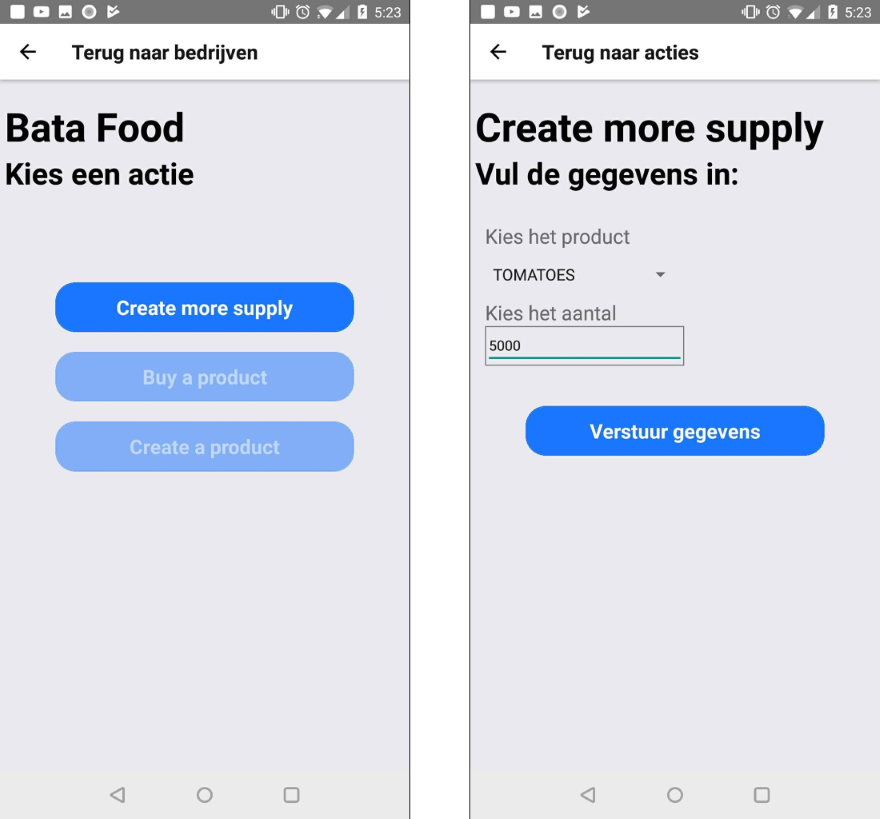
\includegraphics[width=11cm]{img/react-demo-1-2}\\[1cm]
	...
\end{center}

\begin{center}
	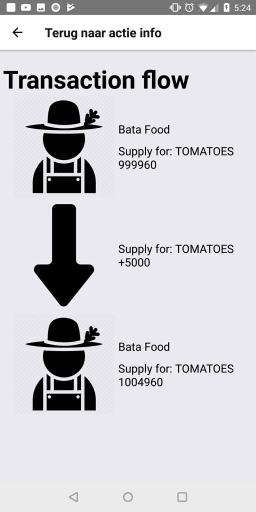
\includegraphics[width=5cm]{img/react-demo-1-3}\\[1cm]
\end{center}

\textbf{Demonstratie 2}

\begin{center}
	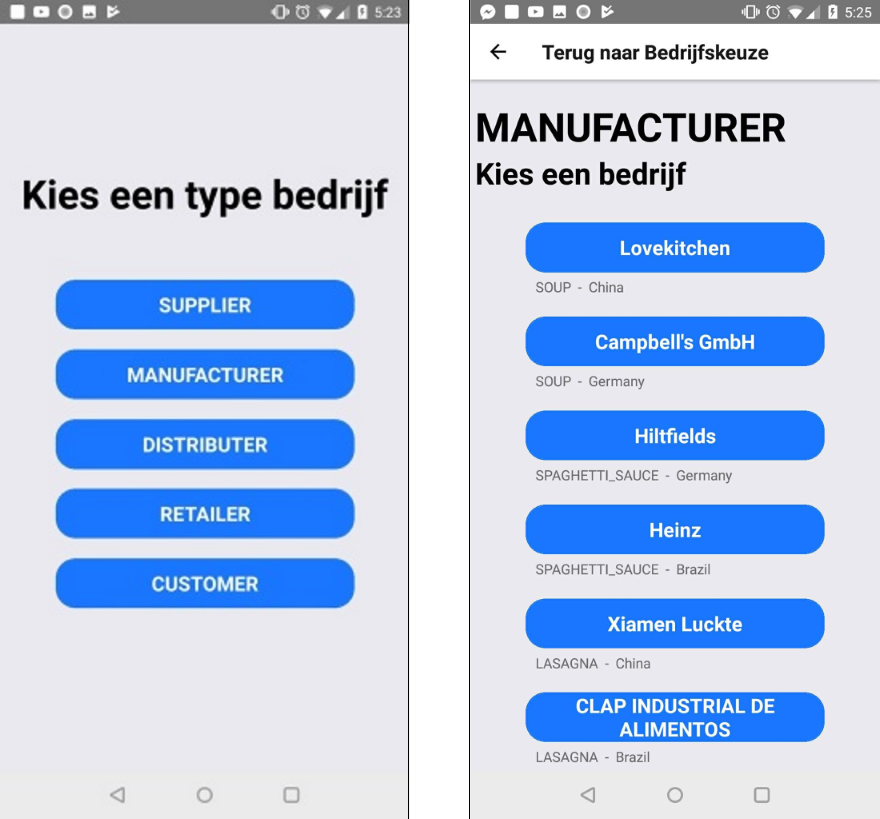
\includegraphics[width=10cm]{img/react-demo-2-1}\\[1cm]
	...
\end{center}
\begin{center}
	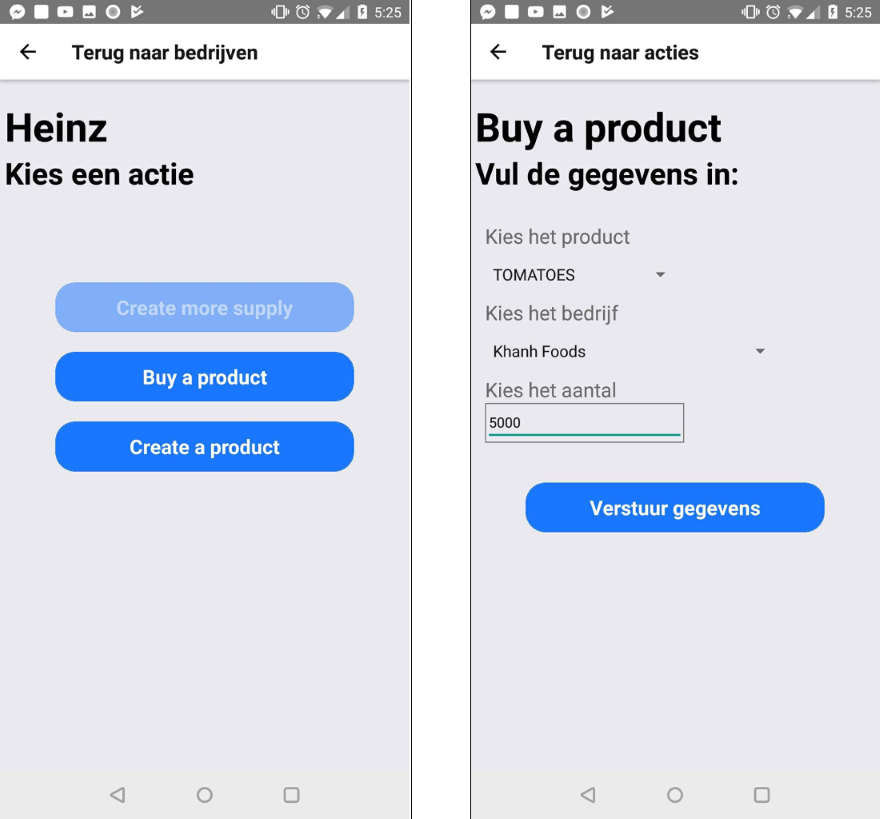
\includegraphics[width=10cm]{img/react-demo-2-2}\\[1cm]
	...
\end{center}
\begin{center}
	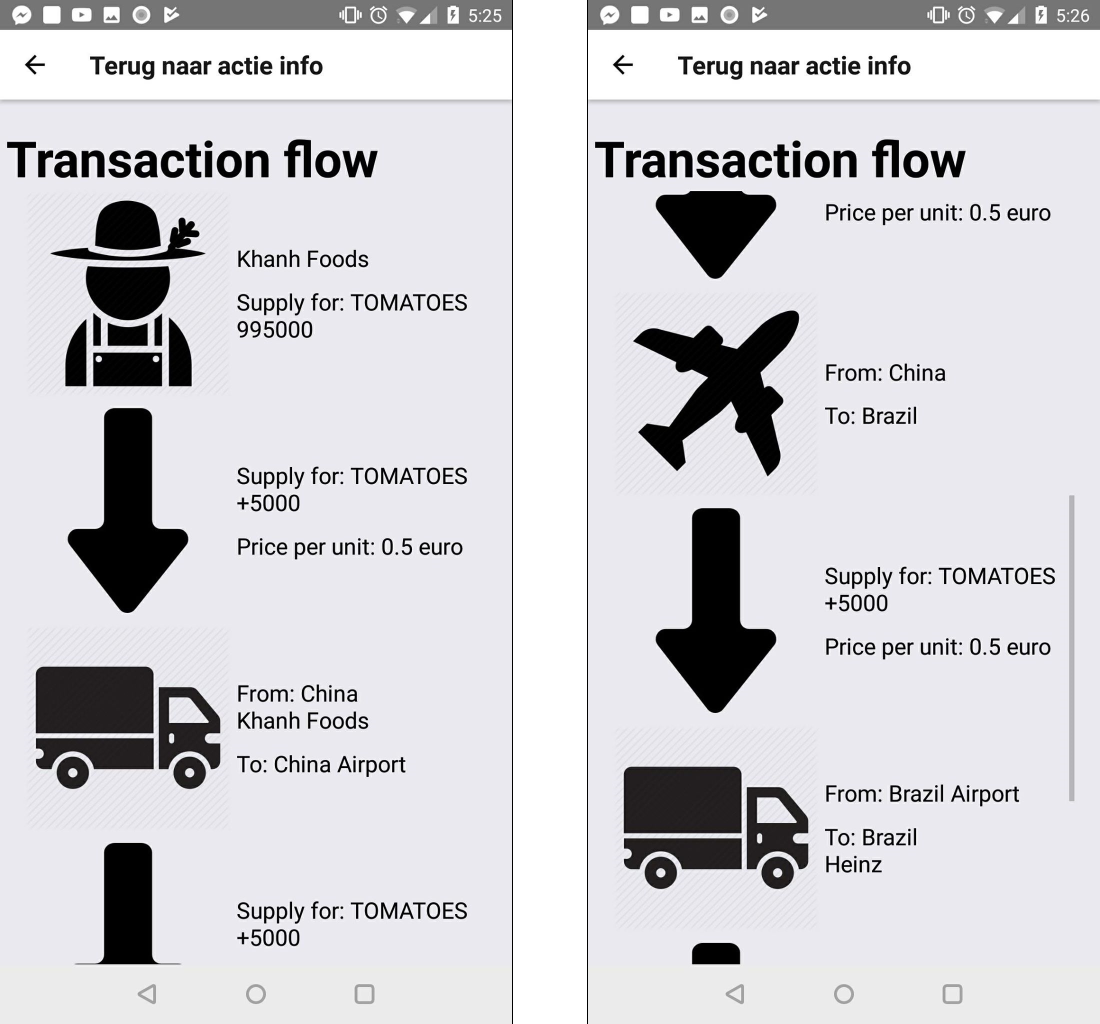
\includegraphics[width=11cm]{img/react-demo-2-3}\\[1cm]
	...
\end{center}
\begin{center}
	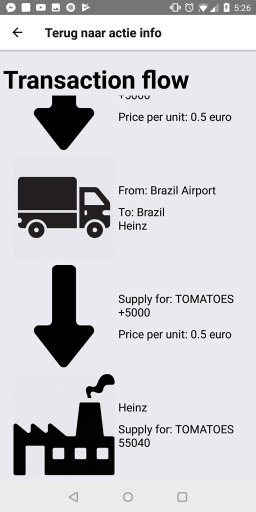
\includegraphics[width=5cm]{img/react-demo-2-4}\\[1cm]
\end{center}

\textbf{Demonstratie 3}

\begin{center}
	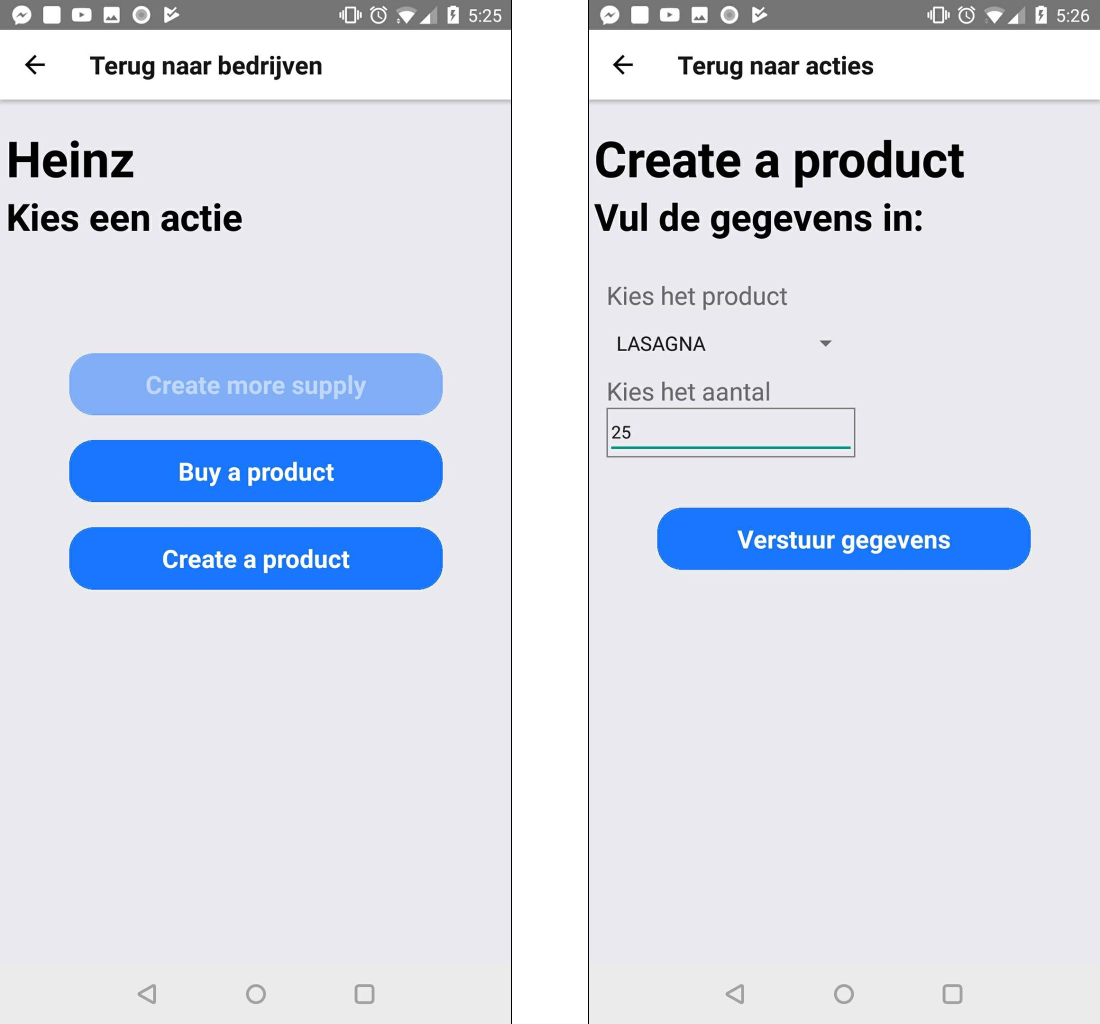
\includegraphics[width=10cm]{img/react-demo-3-1}\\[1cm]
	...
\end{center}
\begin{center}
	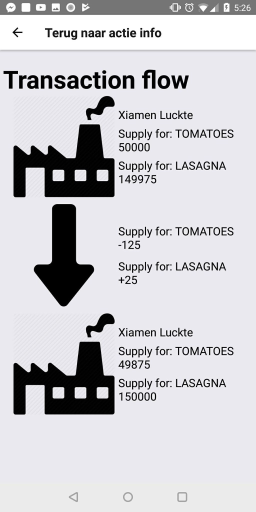
\includegraphics[width=5cm]{img/react-demo-3-2}\\[1cm]
\end{center}


\section{Resultaten testen}
\textbf{creatie van producten in één lijst}
\begin{center}
	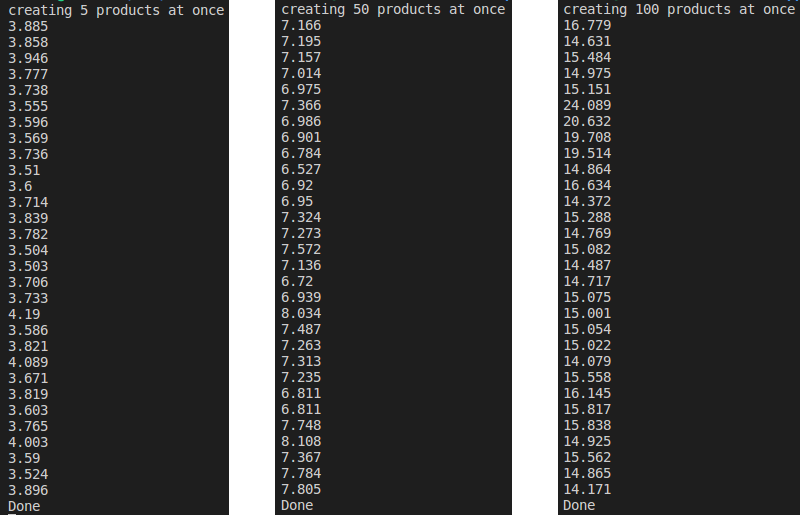
\includegraphics[width=14cm]{img/test-result-1}\\[1cm]
\end{center}
\textbf{creatie van producten elk apart}
\begin{center}
	\includegraphics[width=10cm]{img/test-result-2}\\[1cm]
\end{center}
\textbf{verwijderen van producten in één lijst}
\begin{center}
	\includegraphics[width=12cm]{img/test-result-3}\\[1cm]
\end{center}
\textbf{Ophalen van alle producten}
\begin{center}
	\includegraphics[width=14cm]{img/test-result-4}\\[1cm]
\end{center}
\textbf{Ophalen van één bepaalde ID}
\begin{center}
	\includegraphics[width=14cm]{img/test-result-5}\\[1cm]
\end{center}
\textbf{Ophalen van één bepaalde ID}
\begin{center}
	\includegraphics[width=12cm]{img/test-result-6}\\[1cm]
\end{center}
\section{Netwerk data}
\begin{center}
	\begin{tabular}{ | c | c | c | c |}
		\hline
		\textbf{Soort bedrijf} & \textbf{Naam bedrijf} & \textbf{Land} & \textbf{Product} \\ \hline
		SUPPLIER & Zhengyuan & China & SEEDS \\ \hline
		SUPPLIER & Reimer Seeds & Duitsland & SEEDS \\ \hline
		SUPPLIER & Basso Semillas & Brazilië & SEEDS \\ \hline
		SUPPLIER & Khanh Foods & China & TOMATOES \\ \hline
		SUPPLIER & Silbury & Duitsland & TOMATOES \\ \hline
		SUPPLIER & Bata Food & Brazilië & TOMATOES \\ \hline
		SUPPLIER & Seawinner & China & FERTILIZER \\ \hline
		SUPPLIER & Argus Fertilizer & Brazilië & FERTILIZER \\ \hline
		SUPPLIER & Soil supplier 1 & China & SOIL \\ \hline
		SUPPLIER & Soil supplier 2 & Brazilië & SOIL \\ \hline
		SUPPLIER & Amprion & Duitsland & ELEKTRICITY \\ \hline
		SUPPLIER & Berlin Water Works & Duitsland & WATER \\ \hline
		SUPPLIER & Weidemann GmbH & Duitsland & MACHINES \\ \hline
		SUPPLIER & Schoeller Allibert & Duitsland & CONTAINERS \\ \hline
	\end{tabular}
\end{center}
\begin{center}
	\begin{tabular}{ | c | c | c | c |}
		\hline
		\textbf{Soort bedrijf} & \textbf{Naam bedrijf} & \textbf{Land} & \textbf{Product} \\ \hline
		MANUFACTURER & Lovekitchen & China & SOUP \\ \hline
		MANUFACTURER & Campbell's GmbH & Duitsland & SOUP \\ \hline
		MANUFACTURER & Hiltfields & Duitsland & SPAGHETTI SAUCE \\ \hline
		MANUFACTURER & Heinz & Brazilië & SPAGHETTI SAUCE \\ \hline
		MANUFACTURER & ALIMENTOS & Brazilië & LASAGNA \\ \hline
		MANUFACTURER & Xiamen Luckte & China & LASAGNA \\ \hline
		MANUFACTURER & Tianz & China & KETCHUP \\ \hline
		MANUFACTURER & Hiltfields & Duitsland & KETCHUP \\ \hline
	\end{tabular}
\end{center}
\begin{center}
	\begin{tabular}{ | c | c | c | c |}
		\hline
		\textbf{Soort bedrijf} & \textbf{Naam bedrijf} & \textbf{Land} & \textbf{Product} \\ \hline
		DISTRIBUTER & DISTRIBUTER SAMPLE 1 & Brazilië & PLANE \\ \hline
		DISTRIBUTER & DISTRIBUTER SAMPLE 2 & China & PLANE \\ \hline
		DISTRIBUTER & DISTRIBUTER SAMPLE 3 & Duitsland & PLANE \\ \hline
		DISTRIBUTER & DISTRIBUTER SAMPLE 4 & China & PLANE \\ \hline
		DISTRIBUTER & DISTRIBUTER SAMPLE 5 & Duitsland & PLANE \\ \hline
		DISTRIBUTER & DISTRIBUTER SAMPLE 6 & Brazilië & PLANE \\ \hline
		DISTRIBUTER & DISTRIBUTER SAMPLE 7 & China & CAR \\ \hline
		DISTRIBUTER & DISTRIBUTER SAMPLE 8 & China & CAR \\ \hline
		DISTRIBUTER & DISTRIBUTER SAMPLE 9 & Duitsland & CAR \\ \hline
		DISTRIBUTER & DISTRIBUTER SAMPLE 10 & Duitsland & CAR \\ \hline
		DISTRIBUTER & DISTRIBUTER SAMPLE 11 & Brazilië & CAR \\ \hline
		DISTRIBUTER & DISTRIBUTER SAMPLE 12 & Brazilië & CAR \\ \hline
	\end{tabular}
\end{center}
\begin{center}
	\begin{tabular}{ | c | c | c | c |}
		\hline
		\textbf{Soort bedrijf} & \textbf{Naam bedrijf} & \textbf{Land} & \textbf{Product} \\ \hline
		RETAILER & COLRUYT  & Duitsland & SPAGHETTI SAUCE \\ \hline
		RETAILER & WALMARKT  & Brazilië & SOUP \\ \hline
		RETAILER & PRISMA  & China & LASAGNA \\ \hline
		RETAILER & PANOS  & Duitsland & TOMATOES \\ \hline
		RETAILER & FRITUUR T'HOEKSKE  & Duitsland & KETCHUP \\ \hline
	\end{tabular}
\end{center}
\begin{center}
	\begin{tabular}{ | c | c | c | c |}
		\hline
		\textbf{Soort bedrijf} & \textbf{Naam bedrijf} & \textbf{Land} & \textbf{Product} \\ \hline
		CUSTOMER & Wouter Van Hecke  & China & SPAGHETTI SAUCE \\ \hline
		CUSTOMER & Jens Mortier  & China & SOUP \\ \hline
		CUSTOMER & Hadrien Van Durme  & Duitsland & LASAGNA \\ \hline
		CUSTOMER & Sam Maesschalck  & Duitsland & TOMATOES \\ \hline
		CUSTOMER & Diego Carboni  & Brazilië & KETCHUP \\ \hline
	\end{tabular}
\end{center}

%%---------- Referentielijst --------------------------------------------------

\printbibliography[heading=bibintoc]
%\addcontentsline{toc}{chapter}{\textcolor{maincolor}{\IfLanguageName{dutch}{Bibliografie}{Bibliography}}}

\end{document}
